% =============================================================================
%  RAPPORT DE STAGE — Spécialité Froid et climatisation
%  Thème : Plomberie sanitaire
%  Personnaliser : config/infos.tex  ·  Consignes : ../AGENTS.md
% =============================================================================
\documentclass[12pt,a4paper,oneside]{report}

% =============================================================================
%  PRÉAMBULE : packages
% =============================================================================
\usepackage[T1]{fontenc}
\usepackage[utf8]{inputenc}
\usepackage[french]{babel}
\usepackage[scaled=0.95]{helvet}          % police sans empattement (type Arial)
\renewcommand{\familydefault}{\sfdefault}
\usepackage[a4paper,top=3cm,bottom=2.8cm,left=2.5cm,right=2.5cm,headheight=28pt,footskip=36pt]{geometry}
\usepackage{setspace}
\onehalfspacing
\setlength{\parindent}{0.8cm}
\setlength{\parskip}{4pt}

\usepackage[table]{xcolor}
\usepackage{graphicx}
\usepackage{tikz}
\usetikzlibrary{arrows.meta,positioning,shapes.geometric,calc,fit,shadows,decorations.pathmorphing}
\usepackage[most]{tcolorbox}
\usepackage{array,tabularx,longtable,booktabs,multirow}
\usepackage{float}
\usepackage[labelsep=colon,font={small,it,bf},justification=centering]{caption}
\captionsetup[table]{position=top}
\usepackage{enumitem}
\usepackage{amsmath,amssymb}
\usepackage[locale=FR]{siunitx}
\usepackage{fancyhdr}
\usepackage{titlesec}
\usepackage[titles]{tocloft}
\usepackage{shorttoc}
\usepackage{pdflscape}
\usepackage{csquotes}
\usepackage[backend=biber,style=numeric,sorting=none]{biblatex}
\addbibresource{bib/references.bib}
\usepackage[hidelinks,bookmarksnumbered]{hyperref}

% =============================================================================
%  STYLE : couleurs, bannières vertes, en-tête et pied de page, titres, tables
% =============================================================================
\usepackage{etoc}

% --- Couleurs ----------------------------------------------------------------
\definecolor{vertnuit}{HTML}{1B4D1F}
\definecolor{vertfonce}{HTML}{2E7D32}
\definecolor{vertmoyen}{HTML}{66BB6A}
\definecolor{vertclair}{HTML}{DCEFD9}
\definecolor{bandeau}{HTML}{DDE1F0}
\definecolor{acompleter}{HTML}{E65100}

% --- Champ à compléter -------------------------------------------------------
\newcommand{\AC}[1]{\textcolor{acompleter}{[À COMPLÉTER : #1]}}

% --- Bannière verte (titres liminaires et intercalaires) ---------------------
\newcommand{\banniere}[1]{%
  \begin{center}
  \begin{tikzpicture}
    \node[draw=vertfonce, line width=1.2pt, rounded corners=10pt,
          top color=vertclair, bottom color=vertmoyen!70,
          text=vertnuit, font=\Large\bfseries, align=center,
          inner xsep=22pt, inner ysep=9pt, drop shadow={opacity=0.25}] (b) {#1};
    \foreach \s in {west,east}{
      \fill[vertfonce] (b.\s) circle (5pt);
      \fill[vertclair] (b.\s) circle (2.2pt);
    }
  \end{tikzpicture}
  \end{center}}

% --- Ruban vert du numéro de page --------------------------------------------
\newcommand{\ruban}[1]{%
  \tikz[baseline=(r.base)]{
    \node[fill=vertfonce, text=white, font=\small\bfseries,
          minimum width=1.2cm, inner ysep=3pt] (r) {#1};
    \fill[vertfonce] (r.north east) -- ++(0.35,0) -- ($(r.east)+(0.15,0)$)
                     -- ($(r.south east)+(0.35,0)$) -- (r.south east) -- cycle;
    \fill[vertfonce] (r.north west) -- ++(-0.35,0) -- ($(r.west)+(-0.15,0)$)
                     -- ($(r.south west)+(-0.35,0)$) -- (r.south west) -- cycle;
  }}

% --- En-tête et pied de page -------------------------------------------------
\newcommand{\enteteRapport}{%
  \colorbox{bandeau}{\parbox{\dimexpr\textwidth-2\fboxsep\relax}{\centering
    \footnotesize\bfseries\itshape \InfoTheme{} -- cas de \InfoEntrepriseSigle{}
    au chantier \InfoChantier}}}
\newcommand{\styleRapport}{%
  \fancyhf{}%
  \fancyhead[C]{\enteteRapport}%
  \fancyfoot[L]{\footnotesize\bfseries\itshape Rédigé et présenté par \InfoEtudiantCourt}%
  \fancyfoot[R]{\ruban{\thepage}}%
  \renewcommand{\headrulewidth}{0pt}%
  \renewcommand{\footrulewidth}{0.4pt}}
\pagestyle{fancy}\styleRapport
\fancypagestyle{plain}{\styleRapport}

% --- Numérotation : PARTIE > I. > 1. > a) ------------------------------------
\setcounter{secnumdepth}{3}
\setcounter{tocdepth}{3}
\renewcommand{\thesection}{\Roman{section}.}
\renewcommand{\thesubsection}{\arabic{subsection}.}
\renewcommand{\thesubsubsection}{\alph{subsubsection})}
\counterwithout{figure}{chapter}
\counterwithout{table}{chapter}
\counterwithout{equation}{chapter}
\renewcommand{\thefigure}{\arabic{figure}}
\renewcommand{\thetable}{\arabic{table}}
\renewcommand{\theequation}{\arabic{equation}}

\titleformat{\section}{\normalfont\large\bfseries\color{vertnuit}}{\thesection}{0.5em}{}
\titleformat{\subsection}{\normalfont\normalsize\bfseries\color{vertfonce}}{\thesubsection}{0.5em}{}
\titleformat{\subsubsection}{\normalfont\normalsize\bfseries\itshape}{\thesubsubsection}{0.5em}{}
\titlespacing*{\section}{0pt}{14pt}{6pt}
\titlespacing*{\subsection}{0pt}{10pt}{4pt}
\titlespacing*{\subsubsection}{0pt}{8pt}{3pt}

% --- Pages titrées non numérotées (liminaires, introduction, conclusion…) ----
\newcommand{\pageTitre}[1]{%
  \clearpage\phantomsection
  \addcontentsline{toc}{chapter}{#1}%
  \banniere{#1}\vspace{0.6em}}

% --- Intercalaire de partie --------------------------------------------------
\newcommand{\partie}[2]{%
  \clearpage\setcounter{section}{0}\phantomsection
  \addcontentsline{toc}{chapter}{#1 : #2}%
  \vspace*{\fill}
  \banniere{#1 :\\[4pt] #2}
  \vspace*{\fill}\clearpage}

\newcommand{\conclusionPartielle}{%
  \par\medskip\begin{center}\textbf{\underline{Conclusion partielle}}\end{center}}

% --- Tables des matières, figures, tableaux ----------------------------------
\renewcommand{\cftchapfont}{\bfseries}
\renewcommand{\cftchappagefont}{\bfseries}
\renewcommand{\cftchapleader}{\cftdotfill{\cftdotsep}}
\setlength{\cftbeforechapskip}{4pt}
\setlength{\cftsecnumwidth}{2.6em}
\setlength{\cftsubsecnumwidth}{2em}
\setlength{\cftsubsubsecnumwidth}{2em}
\renewcommand{\cftfigpresnum}{Figure~}
\renewcommand{\cftfigaftersnum}{~:}
\setlength{\cftfignumwidth}{5.6em}
\setlength{\cftfigindent}{0pt}
\renewcommand{\cfttabpresnum}{Tableau~}
\renewcommand{\cfttabaftersnum}{~:}
\setlength{\cfttabnumwidth}{6.2em}
\setlength{\cfttabindent}{0pt}
% Listes des figures et des tableaux : bannière + liste, sans \chapter* ni saut de page
\makeatletter
\AtBeginDocument{%
  \renewcommand{\listoffigures}{\banniere{LISTE DES FIGURES}\vspace{0.4em}\@starttoc{lof}}%
  \renewcommand{\listoftables}{\banniere{LISTE DES TABLEAUX}\vspace{0.4em}\@starttoc{lot}}}
\makeatother

% --- Tableaux ----------------------------------------------------------------
\newcolumntype{Y}{>{\raggedright\arraybackslash}X}
\newcommand{\entete}{\rowcolor{vertclair}}
\renewcommand{\arraystretch}{1.25}

% --- Listes ------------------------------------------------------------------
\setlist[itemize]{label=\textcolor{vertfonce}{\small$\blacklozenge$}, leftmargin=1.4cm, itemsep=2pt, topsep=3pt}
\setlist[enumerate]{leftmargin=1.4cm, itemsep=2pt, topsep=3pt}

% --- Figure factice ou réelle : \figureimg{fichier}{largeur}{légende}{label} --
\newcommand{\figureimg}[4]{%
  \begin{figure}[H]\centering
    \includegraphics[width=#2]{#1}
    \caption{#3}\label{#4}
  \end{figure}}

% =============================================================================
%  INFORMATIONS DU RAPPORT : le SEUL fichier à modifier pour personnaliser.
%  Remplacer chaque \AC{...} par la vraie valeur (sans \AC).
%  \AC{x} s'affiche en orange : [À COMPLÉTER : x]
% =============================================================================

% --- Stagiaire --------------------------------------------------------------
\newcommand{\InfoEtudiant}{\AC{NOM et Prénoms du stagiaire}}
\newcommand{\InfoEtudiantCourt}{\AC{NOM Prénom}}   % pied de page

% --- Formation ---------------------------------------------------------------
\newcommand{\InfoCFP}{\AC{Nom du centre de formation professionnelle}}
\newcommand{\InfoCFPSigle}{\AC{CFP}}
\newcommand{\InfoSpecialite}{Froid et climatisation}
\newcommand{\InfoDiplome}{\AC{Diplôme préparé (ex. DQP)}}
\newcommand{\InfoAnneeEtude}{\AC{Année d'étude (ex. 2\textsuperscript{e} année)}}
\newcommand{\InfoSession}{\AC{Session (ex. 2026)}}

% --- Entreprise d'accueil ----------------------------------------------------
\newcommand{\InfoEntreprise}{\AC{Raison sociale de l'entreprise}}
\newcommand{\InfoEntrepriseSigle}{\AC{SIGLE}}
\newcommand{\InfoEntrepriseVille}{\AC{Ville}}
\newcommand{\InfoEntrepriseQuartier}{\AC{Quartier, repères}}
\newcommand{\InfoEntrepriseCreation}{\AC{année de création}}
\newcommand{\InfoEntrepriseDirigeant}{\AC{Nom du directeur général}}
\newcommand{\InfoEntrepriseCapital}{\AC{capital social en F CFA}}
\newcommand{\InfoEntrepriseEffectif}{\AC{effectif}}
\newcommand{\InfoEntrepriseContact}{\AC{BP, téléphone, courriel, site web}}

% --- Chantier ----------------------------------------------------------------
\newcommand{\InfoChantier}{\AC{Nom du chantier}}
\newcommand{\InfoChantierVille}{\AC{Ville du chantier}}
\newcommand{\InfoChantierNiveaux}{\AC{R+N}}

% --- Encadrement -------------------------------------------------------------
\newcommand{\InfoTuteurAcad}{\AC{M./Mme NOM Prénom}}
\newcommand{\InfoTuteurAcadPoste}{\AC{Poste (ex. formateur en froid et climatisation)}}
\newcommand{\InfoTuteurPro}{\AC{M./Mme NOM Prénom}}
\newcommand{\InfoTuteurProPoste}{\AC{Poste (ex. conducteur des travaux)}}

% --- Stage -------------------------------------------------------------------
\newcommand{\InfoDateDebut}{\AC{date de début}}
\newcommand{\InfoDateFin}{\AC{date de fin}}
\newcommand{\InfoDuree}{quatre (04) mois}

% --- Thème -------------------------------------------------------------------
\newcommand{\InfoTheme}{Plomberie sanitaire}
\newcommand{\InfoSousTheme}{Distribution d'eau froide et d'eau chaude sanitaire dans un immeuble à étages}


\hypersetup{pdftitle={Rapport de stage -- Plomberie sanitaire},
            pdfsubject={Spécialité Froid et climatisation}}

\begin{document}

% ---------------------------------------------------------------- Couverture
% =============================================================================
%  COUVERTURE — jamais paginée. Champs exigés par le cours (module 2, §1) :
%  stagiaire, titre, type de rapport, responsables pro/académique (nom + poste),
%  noms et logos entreprise/centre, formation/diplôme, année d'étude, période.
% =============================================================================
\begin{titlepage}
\thispagestyle{empty}
\begin{tikzpicture}[remember picture,overlay]
  \draw[vertfonce,line width=2.5pt]
    ($(current page.north west)+(1.2cm,-1.2cm)$) rectangle ($(current page.south east)+(-1.2cm,1.2cm)$);
  \draw[vertmoyen,line width=0.8pt]
    ($(current page.north west)+(1.45cm,-1.45cm)$) rectangle ($(current page.south east)+(-1.45cm,1.45cm)$);
\end{tikzpicture}
\singlespacing\centering\vspace*{-1.4cm}

{\scriptsize
\begin{minipage}[t]{0.42\textwidth}\centering
  \textbf{RÉPUBLIQUE DU CAMEROUN}\\ Paix -- Travail -- Patrie\\ \rule{1.5cm}{0.3pt}\\
  \textbf{MINISTÈRE DE L'EMPLOI ET DE LA FORMATION PROFESSIONNELLE}\\ \rule{1.5cm}{0.3pt}\\
  Direction de la Formation et de l'Orientation Professionnelles
\end{minipage}\hfill
\begin{minipage}[t]{0.42\textwidth}\centering
  \textbf{REPUBLIC OF CAMEROON}\\ Peace -- Work -- Fatherland\\ \rule{1.5cm}{0.3pt}\\
  \textbf{MINISTRY OF EMPLOYMENT AND VOCATIONAL TRAINING}\\ \rule{1.5cm}{0.3pt}\\
  Department of Vocational Training and Guidance
\end{minipage}}

\vspace{0.5cm}
\begin{minipage}[c]{0.3\textwidth}\centering
  
\includegraphics[height=2.4cm]{img/logo_cfp.png}\\[2pt]{\scriptsize\InfoCFP}
\end{minipage}\hfill
\begin{minipage}[c]{0.36\textwidth}\centering
  \textbf{\small EXAMENS NATIONAUX DE FIN DE CYCLE DE FORMATION PROFESSIONNELLE}
\end{minipage}\hfill
\begin{minipage}[c]{0.3\textwidth}\centering
  
\includegraphics[height=2.4cm]{img/logo_entreprise.png}\\[2pt]{\scriptsize\InfoEntreprise}
\end{minipage}

\vspace{0.6cm}
{\large\bfseries RAPPORT DE STAGE DE FIN DE FORMATION\par}
\vspace{0.3cm}
\begin{tikzpicture}
  \node[draw=vertfonce,line width=1.5pt,rounded corners=12pt,
        top color=vertclair,bottom color=vertmoyen!70,text=vertnuit,
        align=center,inner xsep=20pt,inner ysep=10pt,text width=12.5cm]
  {{\large\bfseries Thème : \MakeUppercase{\InfoTheme}}\\[4pt]
   {\normalsize\InfoSousTheme}\\[4pt]
   {\normalsize Cas de : \InfoEntrepriseSigle{} au chantier \InfoChantier}};
\end{tikzpicture}

\vspace{0.5cm}
{\normalsize Rapport de stage effectué à \InfoEntreprise\\
du \InfoDateDebut{} au \InfoDateFin{} (\InfoDuree)\par}
\vspace{0.3cm}
{\normalsize\textbf{SPÉCIALITÉ : \MakeUppercase{\InfoSpecialite}}\\
Formation : \InfoDiplome{} \;--\; \InfoAnneeEtude\par}

\vspace{0.6cm}
{\normalsize Rédigé et présenté par :\\[2pt]
{\large\bfseries \InfoEtudiant}\\ Apprenant au \InfoCFPSigle\par}

\vspace{0.6cm}
\begin{minipage}[t]{0.46\textwidth}\centering
  \textbf{\underline{RESPONSABLE ACADÉMIQUE}}\\[3pt]
  \InfoTuteurAcad\\ {\small\itshape\InfoTuteurAcadPoste}
\end{minipage}\hfill
\begin{minipage}[t]{0.46\textwidth}\centering
  \textbf{\underline{RESPONSABLE PROFESSIONNEL}}\\[3pt]
  \InfoTuteurPro\\ {\small\itshape\InfoTuteurProPoste}
\end{minipage}

\vfill
\tikz\node[fill=vertfonce,text=white,font=\bfseries,rounded corners=6pt,inner xsep=14pt,inner ysep=5pt]{Session \InfoSession};
\end{titlepage}


% ------------------------------------------------- Pages liminaires (i, ii…)
\pagenumbering{roman}
\pageTitre{DÉDICACE}
\vspace*{\fill}
\begin{center}
  {\Large\itshape À\\[0.6em] \textbf{mes parents},\\[0.6em]
  pour leur amour, leurs sacrifices et leur soutien constant.}
\end{center}
\vspace*{\fill}


\clearpage\phantomsection
\addcontentsline{toc}{chapter}{SOMMAIRE}
\etocsettocstyle{\banniere{SOMMAIRE}\vspace{0.4em}}{}
\etocsetnexttocdepth{section}
\tableofcontents

\pageTitre{REMERCIEMENTS}

Au terme de ce stage, nous tenons à exprimer notre profonde gratitude à toutes les personnes
qui ont contribué à son bon déroulement et à la rédaction de ce rapport. Nous adressons nos
remerciements en premier lieu :

\begin{itemize}
  \item à \InfoTuteurPro, \InfoTuteurProPoste, notre responsable professionnel, pour son accueil,
        sa disponibilité, la qualité de son encadrement sur le chantier et la confiance qu'il nous
        a accordée ;
  \item à \InfoTuteurAcad, \InfoTuteurAcadPoste, notre responsable académique, pour ses conseils
        méthodologiques, son suivi et ses orientations pendant la rédaction de ce rapport ;
  \item à \InfoEntrepriseDirigeant, Directeur Général de \InfoEntreprise, pour nous avoir ouvert
        les portes de son entreprise ;
  \item au promoteur et à l'ensemble du corps enseignant du \InfoCFP, pour la formation théorique
        et pratique reçue.
\end{itemize}

Nos remerciements vont également :

\begin{itemize}
  \item aux chefs de division, chefs d'équipe, techniciens et manœuvres de \InfoEntrepriseSigle,
        pour leur esprit de partage et leur patience au quotidien ;
  \item à nos camarades de promotion, pour l'entraide et les échanges ;
  \item à notre famille et à nos proches, pour leur soutien moral, matériel et financier tout au
        long de notre formation.
\end{itemize}

Que tous ceux qui, de près ou de loin, ont contribué à la réalisation de ce travail trouvent
ici l'expression de notre sincère reconnaissance.

\pageTitre{LISTE DES ABRÉVIATIONS}

\begin{center}
\begin{tabularx}{0.92\textwidth}{>{\bfseries}l Y}
\toprule
\entete Abréviation & Signification \\
\midrule
AFNOR & Association française de normalisation \\
CFP   & Centre de formation professionnelle \\
DN    & Diamètre nominal \\
DTU   & Document technique unifié \\
ECS   & Eau chaude sanitaire \\
EF    & Eau froide \\
EPI   & Équipement de protection individuelle \\
EU / EV & Eaux usées / eaux vannes \\
FFOM  & Forces, faiblesses, opportunités, menaces \\
HSE   & Hygiène, sécurité et environnement \\
MINEFOP & Ministère de l'Emploi et de la Formation professionnelle \\
PE    & Polyéthylène \\
PER   & Polyéthylène réticulé \\
PN    & Pression nominale \\
PPR   & Polypropylène random (copolymère) \\
PVC   & Polychlorure de vinyle \\
R+N   & Rez-de-chaussée plus N étages \\
SARL  & Société à responsabilité limitée \\
\bottomrule
\end{tabularx}
\end{center}


\clearpage\phantomsection
\addcontentsline{toc}{chapter}{LISTE DES TABLEAUX}
\listoftables

\clearpage\phantomsection
\addcontentsline{toc}{chapter}{LISTE DES FIGURES}
\listoffigures

\pageTitre{AVANT-PROPOS}

La formation professionnelle, telle qu'elle est organisée au Cameroun par le Ministère de
l'Emploi et de la Formation professionnelle (MINEFOP), repose sur l'approche par compétences.
Elle associe l'acquisition de connaissances théoriques, l'apprentissage des gestes
professionnels en atelier et une immersion en entreprise. Le stage de fin de formation en est
l'aboutissement : il confronte l'apprenant aux réalités d'un chantier, à ses contraintes de
délais, de qualité et de sécurité, et à la vie d'une équipe de travail.

C'est dans ce cadre que nous avons effectué un stage de \InfoDuree{} au sein de
\InfoEntreprise, du \InfoDateDebut{} au \InfoDateFin. Affecté à la division plomberie sur le
chantier \InfoChantier, nous avons participé à la pose des réseaux de distribution d'eau froide
et d'eau chaude sanitaire, à l'installation des organes de régulation de pression et à
l'isolation des canalisations.

Bien que notre spécialité soit le froid et la climatisation, ce stage nous a montré à quel
point ces métiers sont liés aux fluides du bâtiment : mêmes matériaux, mêmes techniques
d'assemblage, mêmes exigences d'étanchéité et d'isolation thermique. Le présent rapport rend
compte de ce que nous avons observé, appris et réalisé. Il est également une étape de
réflexion sur notre projet professionnel.


% ------------------------------------------------------- Corps (1, 2, 3…)
\clearpage
\pagenumbering{arabic}
\pageTitre{INTRODUCTION}

Le Cameroun connaît depuis plusieurs années une forte croissance de la construction : immeubles
d'habitation, hôtels, bureaux et équipements publics se multiplient dans les grandes villes.
Chacun de ces bâtiments doit être équipé d'installations techniques fiables : distribution
d'eau, évacuation des eaux usées, climatisation, production de froid. Ces corps d'état
secondaires représentent une part importante du coût d'un ouvrage et conditionnent directement
le confort, l'hygiène et la sécurité de ses occupants. Ils créent aussi une demande soutenue en
techniciens qualifiés.

Apprenant en spécialité \textbf{\InfoSpecialite} au \InfoCFP, nous avons choisi d'effectuer
notre stage de fin de formation au sein de \InfoEntreprise{} (\InfoEntrepriseSigle) pour trois
raisons. D'abord, l'entreprise intervient à la fois en climatisation, en plomberie et en
électricité : c'est un cadre idéal pour comprendre comment ces lots s'articulent sur un même
chantier. Ensuite, elle exécute de grands projets, ce qui permet de découvrir l'organisation
d'un chantier d'envergure. Enfin, nous souhaitions consolider nos compétences en travail des
tubes, en assemblage et en essais d'étanchéité, qui sont communes au froid et à la plomberie.

Durant \InfoDuree, nous avons été affecté au chantier \InfoChantier, un immeuble de type
\InfoChantierNiveaux, où \InfoEntrepriseSigle{} assure notamment le lot plomberie sanitaire.
Le thème retenu pour ce rapport est donc la \textbf{plomberie sanitaire}, et plus précisément
la \emph{\MakeLowercase{\InfoSousTheme}}. Ce sujet est d'un intérêt certain : un réseau mal
dimensionné ou mal réalisé provoque des débits insuffisants aux étages, des coups de bélier,
des fuites et des surconsommations. Il se situe en outre à la frontière de notre spécialité,
puisque la distribution d'eau chaude, l'isolation des canalisations et la production d'eau
glacée font appel aux mêmes principes.

Pour rendre compte de cette expérience, le présent rapport s'articule autour de quatre parties.
La \textbf{première partie} présente l'entreprise d'accueil, son organisation et son
environnement. La \textbf{deuxième partie} décrit le déroulement du stage : poste occupé,
planning des activités, résultats et compétences acquises. La \textbf{troisième partie} traite
du thème technique : généralités sur la plomberie sanitaire, dimensionnement d'une colonne de
distribution, matériaux, mise en œuvre et liens avec le froid et la climatisation. La
\textbf{quatrième partie} est consacrée aux critiques et suggestions. Une conclusion générale
dresse le bilan du stage et ouvre sur nos perspectives professionnelles.

\partie{PREMIÈRE PARTIE}{PRÉSENTATION DE L'ENTREPRISE}

% Contenu exigé par le cours (module 2, §8, premier temps) : présentation, organisation
% (organigramme), historique, secteurs, marchés, clients/fournisseurs, concurrence,
% chiffres clés, perspectives (FFOM), mutations technologiques, volonté des dirigeants.

\section{Présentation générale et historique}

\InfoEntreprise{} (\InfoEntrepriseSigle) est une société à responsabilité limitée de droit
camerounais, créée en \InfoEntrepriseCreation{} et dirigée par \InfoEntrepriseDirigeant. Elle
est spécialisée dans les \textbf{lots techniques du bâtiment} : climatisation et ventilation,
plomberie sanitaire, électricité, détection et protection incendie.

Partie d'une petite équipe de techniciens, l'entreprise s'est progressivement structurée
autour de divisions spécialisées pour répondre à des marchés de plus en plus importants :
résidences, hôtels, immeubles de bureaux et bâtiments publics. \AC{Étapes clés de l'historique :
premiers marchés, extension des activités, certifications, grands chantiers réalisés.}

Sa vocation est d'apporter à ses clients une prestation complète, de l'étude à la mise en
service, puis à la maintenance des installations.

\section{Situation géographique}

Le siège de \InfoEntrepriseSigle{} est situé à \InfoEntrepriseVille, au quartier
\InfoEntrepriseQuartier. Sa position dans un quartier accessible facilite l'approvisionnement
en matériel et le déplacement des équipes vers les chantiers. La figure~\ref{fig:localisation}
présente la localisation du siège.

\figureimg{img/fig_localisation}{0.75\textwidth}{plan de localisation du siège de l'entreprise}{fig:localisation}

\section{Missions et domaines d'activité}

\subsection{Missions}
L'entreprise a pour mission de concevoir, réaliser et entretenir les installations techniques
des bâtiments, dans le respect des règles de l'art, des délais et des budgets de ses clients.
Concrètement, elle :
\begin{itemize}
  \item réalise les études techniques et les plans d'exécution des installations ;
  \item fournit et pose les équipements et les réseaux ;
  \item effectue les essais, la mise en service et la réception des ouvrages ;
  \item assure la maintenance préventive et corrective dans le cadre de contrats d'entretien.
\end{itemize}

\subsection{Secteurs d'activité}
Le tableau~\ref{tab:activites} résume les principaux domaines d'intervention.

\begin{table}[H]\centering
\caption{domaines d'activité de l'entreprise}\label{tab:activites}
\begin{tabularx}{\textwidth}{>{\bfseries}p{3.6cm} Y}
\toprule
\entete Domaine & Prestations \\
\midrule
Climatisation & Installation de climatiseurs individuels (split, cassette), systèmes à débit de réfrigérant variable, centrales de traitement d'air, ventilation \\
Froid & Chambres froides positives et négatives, vitrines réfrigérées, maintenance frigorifique \\
Plomberie sanitaire & Réseaux d'eau froide et d'eau chaude, évacuations, appareils sanitaires, surpresseurs, production d'eau chaude \\
Électricité & Courants forts et courants faibles, éclairage, tableaux électriques \\
Sécurité incendie & Détection, extinction, robinets d'incendie armés \\
\bottomrule
\end{tabularx}
\end{table}

\subsection{Savoir-faire et atouts}
L'entreprise s'appuie sur une \textbf{offre multi-lots}, qui permet au client de traiter avec
un interlocuteur unique pour plusieurs corps d'état. Elle dispose d'un personnel
pluridisciplinaire, d'un parc d'outillage spécialisé (polyfuseurs, groupes de soudure, pompes
d'épreuve, pompes à vide) et d'une expérience des chantiers de grande hauteur.

\section{Organisation et organigramme}

\subsection{Organisation générale}
L'entreprise est organisée de façon hiérarchique. La direction générale définit la stratégie
et suit les marchés. La direction technique coordonne les études et l'exécution. Le conducteur
des travaux, également chargé d'études, organise les chantiers. Les chefs de division
(climatisation, plomberie, électricité, réseaux et gaines, génie civil) encadrent les chefs
d'équipe, eux-mêmes responsables des techniciens et des manœuvres. Un magasinier gère les
stocks et un service logistique assure les transports. L'effectif est de
\InfoEntrepriseEffectif{} personnes.

\subsection{Organigramme}
La figure~\ref{fig:organigramme} présente l'organigramme fonctionnel de l'entreprise. Notre
position de stagiaire y est indiquée en vert : nous étions rattaché à l'équipe plomberie, sous
l'autorité du chef de division plomberie.

\begin{figure}[H]\centering
% Organigramme fonctionnel (à adapter à l'entreprise réelle)
\begin{tikzpicture}[
  font=\scriptsize\bfseries, node distance=6mm and 3mm,
  bloc/.style={draw=vertfonce, fill=vertclair, rounded corners=3pt, align=center,
               minimum height=8mm, text width=2.15cm, inner sep=2pt},
  lien/.style={-{Stealth[length=2mm]}, vertfonce, line width=0.6pt}]
  \node[bloc, fill=vertfonce, text=white, text width=3.2cm] (dg) {Directeur général};
  \node[bloc, left=1.4cm of dg] (dt) {Directeur technique};
  \node[bloc, right=1.4cm of dg, text width=2.6cm] (ct) {Conducteur des travaux\\chargé d'études};
  \node[bloc, below=17mm of dg, xshift=-5.0cm] (d1) {Division\\climatisation};
  \node[bloc, right=of d1] (d2) {Division\\plomberie};
  \node[bloc, right=of d2] (d3) {Division\\électricité};
  \node[bloc, right=of d3] (d4) {Division réseaux\\et gaines};
  \node[bloc, right=of d4] (d5) {Division\\génie civil};
  \node[bloc, below=of d1] (e1) {Chef d'équipe\\climatisation};
  \node[bloc, below=of d2] (e2) {Chef d'équipe\\plomberie};
  \node[bloc, below=of d3] (e3) {Chef d'équipe\\électricité};
  \node[bloc, below=of d4] (e4) {Magasinier};
  \node[bloc, below=of d5] (e5) {Logistique\\chauffeur};
  \node[bloc, below=of e2, text width=4.4cm, xshift=1.2cm] (tech) {Techniciens};
  \node[bloc, below=of tech, text width=4.4cm] (man) {Manœuvres};
  \node[bloc, right=6mm of tech, fill=vertmoyen, text=white] (stg) {STAGIAIRE};
  \draw[lien] (dg) -- (dt);
  \draw[lien] (dg) -- (ct);
  \coordinate (bus) at ($(dg.south)+(0,-11mm)$);
  \draw[vertfonce, line width=0.6pt] (dg.south) -- (bus);
  \draw[vertfonce, line width=0.6pt] (bus -| d1.north) -- (bus -| d5.north);
  \foreach \d in {d1,d2,d3,d4,d5} \draw[lien] (bus -| \d.north) -- (\d.north);
  \foreach \d/\e in {d1/e1,d2/e2,d3/e3,d4/e4,d5/e5} \draw[lien] (\d) -- (\e);
  \draw[lien] (e2.south) -- (e2.south |- tech.north);
  \draw[lien] (tech) -- (man);
  \draw[lien, dashed, vertmoyen] (e2.south east) -- (stg.north west);
\end{tikzpicture}

\caption{organigramme fonctionnel de l'entreprise}\label{fig:organigramme}
\end{figure}

\subsection{Personnel d'encadrement rencontré}
\begin{table}[H]\centering
\caption{principaux responsables et leurs postes}\label{tab:membres}
\begin{tabularx}{0.9\textwidth}{Y Y}
\toprule
\entete Nom & Poste \\
\midrule
\InfoEntrepriseDirigeant & Directeur général \\
\AC{Nom} & Directeur technique \\
\InfoTuteurPro & \InfoTuteurProPoste \\
\AC{Nom} & Chef de division plomberie \\
\AC{Nom} & Chef de division climatisation \\
\AC{Nom} & Chef d'équipe plomberie \\
\AC{Nom} & Magasinier \\
\bottomrule
\end{tabularx}
\end{table}

\section{Environnement économique}

\subsection{Marchés et clients}
L'entreprise intervient principalement sur le \textbf{marché du bâtiment neuf} (immeubles
d'habitation, hôtels, bureaux) et sur celui de la \textbf{maintenance}. Ses clients sont des
promoteurs immobiliers privés, des maîtres d'ouvrage publics, des entreprises générales de
bâtiment qui lui sous-traitent les lots techniques, et des établissements (hôtels, banques,
cliniques) liés par des contrats d'entretien. \AC{Exemples de clients et de chantiers de
référence.}

\subsection{Fournisseurs}
Les tubes et raccords (PPR, PVC, PE, cuivre), les appareils sanitaires, les climatiseurs et les
fluides frigorigènes sont achetés auprès de distributeurs locaux, dont une partie importe le
matériel. La disponibilité et le délai de livraison de certaines références constituent un
enjeu pour le respect des plannings. \AC{Principaux fournisseurs.}

\subsection{Situation concurrentielle}
Le secteur des lots techniques est concurrentiel. Il comprend de grandes entreprises
générales, des sociétés spécialisées et de nombreux artisans informels qui pratiquent des prix
bas. \InfoEntrepriseSigle{} se différencie par son offre multi-lots, son expérience des grands
chantiers et sa capacité à assurer la maintenance après livraison.

\subsection{Chiffres clés}
\begin{table}[H]\centering
\caption{chiffres clés de l'entreprise}\label{tab:chiffres}
\begin{tabularx}{0.85\textwidth}{>{\bfseries}p{6cm} Y}
\toprule
\entete Indicateur & Valeur \\
\midrule
Forme juridique & SARL \\
Année de création & \InfoEntrepriseCreation \\
Capital social & \InfoEntrepriseCapital \\
Effectif & \InfoEntrepriseEffectif \\
Chiffre d'affaires annuel & \AC{montant} \\
Zone d'intervention & \AC{villes, régions, pays} \\
Contacts & \InfoEntrepriseContact \\
\bottomrule
\end{tabularx}
\end{table}

\section{Perspectives d'évolution}

\subsection{Analyse FFOM}
Le tableau~\ref{tab:ffom} résume notre analyse des forces, faiblesses, opportunités et menaces
de l'entreprise, établie à partir de nos observations sur le chantier et de nos échanges avec
le personnel.

\begin{table}[H]\centering
\caption{analyse FFOM de l'entreprise}\label{tab:ffom}
\begin{tabularx}{\textwidth}{Y Y}
\toprule
\entete \textbf{Forces} & \textbf{Faiblesses} \\
\midrule
Offre multi-lots (froid, plomberie, électricité) ; personnel expérimenté ; références de grands chantiers ; capacité de maintenance &
Gestion des stocks et des approvisionnements perfectible ; sécurité sur chantier insuffisamment formalisée ; dépendance à quelques gros marchés \\
\midrule
\entete \textbf{Opportunités} & \textbf{Menaces} \\
\midrule
Croissance de la construction urbaine ; demande en efficacité énergétique et en climatisation performante ; contrats de maintenance récurrents &
Concurrence des prestataires informels ; hausse du coût des matériaux importés ; retards de paiement des maîtres d'ouvrage \\
\bottomrule
\end{tabularx}
\end{table}

\subsection{Mutations technologiques et volonté des dirigeants}
Le métier évolue rapidement : généralisation des tubes de synthèse (PPR, PER, multicouche) à la
place de l'acier galvanisé, remplacement progressif des fluides frigorigènes à fort potentiel de
réchauffement global, développement des climatiseurs à technologie \emph{inverter} et des
systèmes à débit de réfrigérant variable. Les dirigeants souhaitent accompagner ces mutations en
formant leur personnel et en développant l'activité de maintenance, plus régulière que celle des
travaux neufs. \AC{Projets annoncés par la direction.}

\conclusionPartielle
\InfoEntrepriseSigle{} est une entreprise structurée, dont l'offre couvre l'ensemble des lots
techniques du bâtiment. Son organisation hiérarchique claire et la diversité de ses activités en
font un cadre propice à l'apprentissage. L'analyse de son environnement montre une entreprise
bien placée sur un marché porteur, mais qui doit renforcer sa logistique et sa culture de la
sécurité. C'est dans ce cadre que s'est déroulé notre stage, dont la deuxième partie rend compte.

\partie{DEUXIÈME PARTIE}{DÉROULEMENT DU STAGE}

% Contenu exigé par le cours (module 2, §8, second temps) : poste occupé, position dans
% l'organigramme, faits importants, objectifs et enjeux, méthodes et moyens, collaborateurs,
% responsabilités, résultats, difficultés et solutions. Éviter le récit au jour le jour.

\section{Accueil, poste occupé et cadre de la mission}

\subsection{Accueil et intégration}
À notre arrivée, nous avons été reçu par \InfoTuteurPro, \InfoTuteurProPoste, qui nous a
présenté l'entreprise, son règlement intérieur et les consignes de sécurité. Après une visite
du siège et du magasin, nous avons été conduit sur le chantier \InfoChantier{} et présenté à
l'équipe plomberie. Nous avons reçu nos équipements de protection individuelle (casque,
chaussures de sécurité, gants, gilet haute visibilité).

\subsection{Poste occupé et position dans l'organigramme}
Nous avons occupé un poste d'\textbf{aide-technicien plombier} au sein de la division plomberie
(figure~\ref{fig:organigramme}). Nous travaillions sous l'autorité directe du chef d'équipe
plomberie, avec deux à trois techniciens et des manœuvres. Le chef de division plomberie et le
conducteur des travaux contrôlaient régulièrement l'avancement et la qualité des ouvrages.

\subsection{Objectifs et enjeux de la mission}
La mission confiée à l'équipe plomberie était de réaliser, dans les délais du planning général,
les réseaux de distribution d'eau froide et d'eau chaude sanitaire des étages, puis de poser
les organes de régulation et de contrôle (réducteurs de pression, manomètres, vannes
d'isolement). Nos objectifs personnels étaient les suivants :
\begin{itemize}
  \item maîtriser la lecture des plans d'exécution et des schémas de principe ;
  \item maîtriser l'assemblage des tubes PPR par polyfusion ;
  \item comprendre le rôle et le réglage des réducteurs de pression ;
  \item participer aux essais d'étanchéité et à la mise en eau ;
  \item découvrir l'organisation d'un chantier de grande hauteur et la coordination entre lots.
\end{itemize}
L'enjeu pour l'entreprise était double : respecter le planning contractuel, dont dépendaient les
corps d'état suivants (carreleurs, peintres, menuisiers), et livrer des réseaux étanches du
premier coup, car toute reprise après la pose des revêtements est coûteuse.

\section{Méthodes et moyens}

\subsection{Organisation du travail}
Chaque semaine, le chef d'équipe recevait du conducteur des travaux les zones à traiter et les
quantités de matériel correspondantes. Le travail était organisé \textbf{étage par étage} :
traçage et repérage, perçage et pose des supports, préparation des tubes, assemblage,
raccordement, puis essai. Une fiche d'autocontrôle était remplie à la fin de chaque zone.

\subsection{Moyens humains et matériels}
\begin{table}[H]\centering
\caption{moyens humains et matériels mobilisés}\label{tab:moyens}
\begin{tabularx}{\textwidth}{>{\bfseries}p{3.4cm} Y}
\toprule
\entete Catégorie & Détail \\
\midrule
Personnel & 1 chef d'équipe, 2 à 3 techniciens plombiers, 2 manœuvres, 1 stagiaire \\
Outillage & Polyfuseur et matrices de 20 à 63 mm, coupe-tubes, clés à molette et clés plates, niveau, mètre, perceuse-perforateur, pompe d'épreuve manuelle \\
Matériaux & Tubes et raccords PPR, flexibles inox, vannes à sphère, réducteurs de pression, manomètres, colliers et supports, isolant à cellules fermées \\
Sécurité & Casque, gants, chaussures de sécurité, lunettes, harnais pour les travaux en hauteur \\
Documents & Plans d'exécution, schémas de principe, fiches techniques des fabricants, fiches d'autocontrôle \\
\bottomrule
\end{tabularx}
\end{table}

\subsection{Personnes avec lesquelles nous avons collaboré}
Nous avons travaillé au quotidien avec le chef d'équipe plomberie et les techniciens de la
division. Nous avons également échangé avec l'équipe climatisation, notamment pour la
coordination des passages de tuyauteries dans les gaines techniques, et avec le magasinier
pour la préparation des sorties de matériel.

\section{Planning des activités menées}

Le tableau~\ref{tab:planning} présente le planning des activités, regroupées par période. La
figure~\ref{fig:gantt} en donne une vue d'ensemble.

\begin{longtable}{p{1.7cm} p{6.0cm} p{4.0cm} p{2.3cm}}
\caption{planning des activités menées}\label{tab:planning}\\
\toprule
\entete \textbf{Semaines} & \textbf{Activités} & \textbf{Outils} & \textbf{Domaine}\\
\midrule\endfirsthead
\toprule
\entete \textbf{Semaines} & \textbf{Activités} & \textbf{Outils} & \textbf{Domaine}\\
\midrule\endhead
\bottomrule\endfoot
S1 & Accueil, sécurité, visite du chantier, lecture des plans & Plans, EPI & Général \\
S2 -- S3 & Inventaire et préparation du matériel, traçage des réseaux aux étages & Mètre, niveau, cordeau & Plomberie \\
S4 -- S6 & Pose des supports et des canalisations PPR d'eau froide et d'eau chaude aux étages supérieurs & Polyfuseur, coupe-tube, perforateur & Plomberie \\
S7 -- S8 & Pose des canalisations aux étages inférieurs, raccordement aux colonnes montantes & Polyfuseur, coupe-tube & Plomberie \\
S9 & Essais d'étanchéité par zone, reprise des fuites & Pompe d'épreuve, manomètre & Plomberie \\
S10 -- S11 & Isolation des canalisations d'eau chaude et des réseaux exposés & Cutter, colle néoprène & Plomberie / Froid \\
S12 -- S13 & Montage des réducteurs de pression et des manomètres dans les locaux techniques et aux étages & Clés à molette, ruban PTFE & Plomberie \\
S14 & Pose des flexibles et de la robinetterie dans les salles d'eau & Clés plates, flexibles & Plomberie \\
S15 & Appui à l'équipe climatisation : pose de liaisons frigorifiques et d'évacuations de condensats & Cintreuse, dudgeonnière & Froid \\
S16 & Mise en eau, réglage des pressions, autocontrôles, bilan du stage & Manomètre & Plomberie \\
\end{longtable}

\begin{figure}[H]\centering
% Diagramme de Gantt du stage (16 semaines), cohérent avec le tableau du planning
\begin{tikzpicture}[x=0.72cm,y=0.55cm,font=\scriptsize]
  \foreach \s in {1,...,16} {
    \node[anchor=south] at (\s-0.5,0.2) {S\s};
    \draw[gray!30] (\s,0) -- (\s,-10);
  }
  \draw[gray!30] (0,0) -- (0,-10);
  \foreach [count=\i] \lib/\deb/\fin/\col in {
      Accueil et sécurité/0/1/vertfonce,
      Préparation et traçage/1/3/vertfonce,
      Canalisations étages hauts/3/6/vertmoyen,
      Canalisations étages bas/6/8/vertmoyen,
      Essais d'étanchéité/8/9/acompleter,
      Isolation des réseaux/9/11/vertfonce,
      Réducteurs et manomètres/11/13/vertmoyen,
      Robinetterie et flexibles/13/14/vertmoyen,
      Appui climatisation/14/15/bandeau!60!blue,
      Mise en eau et bilan/15/16/acompleter} {
    \node[anchor=east] at (-0.15,-\i+0.5) {\lib};
    \fill[\col, rounded corners=1.5pt] (\deb+0.05,-\i+0.15) rectangle (\fin-0.05,-\i+0.85);
  }
\end{tikzpicture}

\caption{vue d'ensemble du planning du stage}\label{fig:gantt}
\end{figure}

\section{Responsabilités, faits marquants et résultats}

\subsection{Responsabilités exercées}
Après une période d'observation, nous avons progressivement pris en charge des tâches
complètes : coupe et assemblage des tubes PPR, montage des réducteurs de pression et des
manomètres sur les colonnes des étages, isolation des réseaux d'eau chaude. Nous étions chargé
de la tenue de la fiche d'autocontrôle de notre zone et de la vérification de la présence du
matériel avant le début des travaux.

\subsection{Faits marquants}
\begin{itemize}
  \item La \textbf{détection d'une fuite} sur un assemblage lors d'un essai de pression : elle
        provenait d'une soudure réalisée avec un temps de chauffe insuffisant. L'assemblage a été
        coupé et refait. Cet incident a montré l'importance du respect des paramètres de soudage.
  \item La constatation d'une \textbf{pression statique trop élevée} aux étages inférieurs, qui
        justifie la pose de réducteurs de pression (voir troisième partie).
  \item Une \textbf{rupture d'approvisionnement} en raccords de 40 mm, qui a retardé une zone de
        deux jours et a conduit l'équipe à réorganiser l'ordre des étages.
\end{itemize}

\subsection{Résultats obtenus}
À la fin du stage, notre équipe avait achevé la distribution d'eau froide et d'eau chaude de
\AC{nombre} niveaux, monté \AC{nombre} réducteurs de pression et manomètres, et isolé environ
\AC{longueur} mètres de canalisations. Tous les réseaux auxquels nous avons participé ont passé
avec succès l'essai d'étanchéité après reprise.

\section{Difficultés rencontrées et solutions apportées}

\begin{table}[H]\centering
\caption{difficultés rencontrées et solutions apportées}\label{tab:difficultes}
\begin{tabularx}{\textwidth}{Y Y}
\toprule
\entete Difficulté & Solution apportée \\
\midrule
Manque de maîtrise initiale de la polyfusion (soudures irrégulières) & Entraînement sur des chutes de tube, respect strict des temps de chauffe affichés par le fabricant \\
Lecture des plans d'exécution de plusieurs niveaux & Accompagnement du chef d'équipe, repérage systématique des cotes et des niveaux \\
Ruptures de stock de certains raccords & Anticipation des besoins par zone, réorganisation de l'ordre des étages \\
Travail en hauteur et zones mal éclairées & Port du harnais, demande de projecteurs de chantier \\
Distance et coût du transport vers le chantier & Organisation du trajet en covoiturage avec des collègues \\
\bottomrule
\end{tabularx}
\end{table}

\section{Compétences acquises}

\subsection{Compétences professionnelles}
\begin{itemize}
  \item Lire un plan d'exécution et un schéma de principe de plomberie ;
  \item Couper, chanfreiner et assembler des tubes PPR par polyfusion ;
  \item Monter et régler un réducteur de pression, installer un manomètre ;
  \item Réaliser un essai d'étanchéité et interpréter la chute de pression ;
  \item Isoler une canalisation avec un isolant à cellules fermées ;
  \item Appliquer les règles de sécurité d'un chantier de grande hauteur.
\end{itemize}

\subsection{Compétences personnelles}
\begin{itemize}
  \item Ponctualité et rigueur dans l'exécution des tâches ;
  \item Travail en équipe et communication avec les autres corps d'état ;
  \item Autonomie et prise d'initiative ;
  \item Gestion du temps et respect des consignes.
\end{itemize}

\conclusionPartielle
Ce stage nous a permis d'occuper une place réelle dans une équipe de production. En passant de
l'observation à l'exécution, nous avons acquis des gestes professionnels précis et compris les
contraintes d'un chantier : délais, coordination, qualité et sécurité. Les difficultés
rencontrées ont été autant d'occasions d'apprendre. La troisième partie approfondit le thème
technique au cœur de ces activités : la plomberie sanitaire.

\partie{TROISIÈME PARTIE}{PLOMBERIE SANITAIRE}

\section{Généralités sur la plomberie sanitaire}

\subsection{Définition et rôle}
La plomberie sanitaire regroupe l'ensemble des installations qui assurent, dans un bâtiment,
l'\textbf{alimentation en eau} des appareils sanitaires (eau froide et eau chaude) et
l'\textbf{évacuation des eaux usées et des eaux vannes} vers le réseau d'assainissement. Elle
doit garantir à chaque point de puisage un débit et une pression suffisants, une eau de
qualité, l'absence de bruit et de fuite, et la sécurité des usagers. En France, ces
installations sont encadrées par le NF DTU~60.1 pour la mise en œuvre et par le NF DTU~60.11
pour les règles de calcul \cite{dtu601,dtu6011}. Ces documents servent couramment de
référence technique au Cameroun.

\subsection{Constitution d'une installation}
Une installation de plomberie sanitaire comprend les éléments suivants
(figure~\ref{fig:principe}) :
\begin{itemize}
  \item le \textbf{branchement} au réseau public, avec le compteur, une vanne d'arrêt et un
        clapet anti-retour ;
  \item le cas échéant, un \textbf{réservoir de stockage (bâche)} et un \textbf{surpresseur},
        lorsque la pression du réseau public est insuffisante pour desservir les étages ;
  \item la \textbf{distribution d'eau froide} (EF) : colonnes montantes, puis distribution par
        étage et par logement ;
  \item la \textbf{production d'eau chaude sanitaire} (ECS) : chauffe-eau électrique,
        chaudière ou système solaire, et la distribution d'ECS ;
  \item les \textbf{organes de régulation et de contrôle} : réducteurs de pression, manomètres,
        vannes d'isolement, purges ;
  \item les \textbf{appareils sanitaires} : lavabos, douches, WC, éviers ;
  \item les \textbf{évacuations} : eaux usées (EU), eaux vannes (EV) et leur ventilation.
\end{itemize}

\begin{figure}[H]\centering
% Schéma de principe : branchement -> bâche -> surpresseur -> colonnes EF/ECS -> étages -> évacuations
\begin{tikzpicture}[font=\scriptsize, >=Stealth,
  eq/.style={draw=vertnuit, fill=vertclair, rounded corners=2pt, align=center, minimum height=8mm, inner sep=3pt},
  app/.style={draw=gray!70, fill=white, align=center, minimum width=10mm, minimum height=5mm, inner sep=1pt},
  ef/.style={blue!70!black, line width=1.2pt},
  ecs/.style={red!75!black, line width=1.2pt},
  eu/.style={brown!70!black, line width=1.6pt, dashed}]
  % Réseau public et branchement
  \node[eq] (pub) at (0,0) {Réseau\\public};
  \node[eq, right=6mm of pub] (cpt) {Compteur\\+ clapet};
  \node[eq, right=6mm of cpt] (bache) {Bâche\\(stockage)};
  \node[eq, right=6mm of bache] (surp) {Surpresseur};
  \draw[ef,->] (pub) -- (cpt);
  \draw[ef,->] (cpt) -- (bache);
  \draw[ef,->] (bache) -- (surp);
  % Colonnes
  \coordinate (cEF) at (8.6,0);
  \coordinate (cECS) at (9.4,0);
  \draw[ef] (surp) -- (cEF);
  \draw[ef,->] (cEF) -- ++(0,5.6) node[above left, inner sep=1pt] {Colonne EF};
  % Production ECS
  \node[eq, fill=red!10] (ce) at (11.2,0.9) {Production\\ECS};
  \draw[ef,->] (cEF |- ce.west) -- (ce.west);
  \draw[ecs] (ce.north) |- (cECS |- 1.8,1.8);
  \draw[ecs,->] (cECS |- 1.8,1.8) -- (cECS |- 5.6,5.6) node[above right, inner sep=1pt] {Colonne ECS};
  % Étages
  \foreach \y/\n/\i in {2.6/R+1/a, 3.8/R+2/b, 5.0/R+N/c} {
    \draw[gray!50] (-0.3,\y-0.45) -- (12.6,\y-0.45);
    \node[anchor=west, gray] at (-0.3,\y) {\n};
    \node[eq, fill=white, minimum height=6mm] (rp\i) at (7.2,\y-0.08) {Réducteur\\+ manomètre};
    \draw[ef,->] (cEF |- rp\i.east) -- (rp\i.east);
    \node[app] (lav\i) at (1.6,\y) {Lavabo};
    \node[app] (dou\i) at (3.0,\y) {Douche};
    \node[app] (wc\i) at (4.4,\y) {WC};
    \draw[ef,->] (rp\i.west) -- (wc\i.east);
    \draw[ecs] (cECS |- 0,\y+0.42) -- (2.2,\y+0.42) -- (2.2,\y+0.3);
    \draw[eu] (4.4,\y-0.25) -- (4.4,\y-0.38) -- (0.75,\y-0.38); \draw[eu] (1.6,\y-0.25) -- (1.6,\y-0.38); \draw[eu] (3.0,\y-0.25) -- (3.0,\y-0.38);
  }
  % Chute EU/EV
  \draw[eu,->] (0.75,4.62) -- (0.75,1.1) node[right, text=brown!70!black] {Chute EU/EV vers l'égout};
  % Légende
  \begin{scope}[shift={(0,-1.6)}]
    \draw[ef] (0,0) -- (0.6,0); \node[anchor=west] at (0.7,0) {Eau froide (EF)};
    \draw[ecs] (3.2,0) -- (3.8,0); \node[anchor=west] at (3.9,0) {Eau chaude sanitaire (ECS)};
    \draw[eu] (7.4,0) -- (8.0,0); \node[anchor=west] at (8.1,0) {Évacuations EU/EV};
  \end{scope}
\end{tikzpicture}

\caption{schéma de principe d'une installation de plomberie sanitaire d'immeuble}\label{fig:principe}
\end{figure}

Le détail de la distribution à l'intérieur d'un logement est donné en
\hyperref[ann:schema]{annexe~1}.

\subsection{Matériaux des canalisations}
Le choix du matériau dépend de l'usage (eau froide, eau chaude, évacuation), de la pression,
de la température et du coût. Le tableau~\ref{tab:materiaux} compare les principaux matériaux
rencontrés sur les chantiers.

\begin{table}[H]\centering
\caption{comparaison des matériaux de canalisation}\label{tab:materiaux}
\begin{tabularx}{\textwidth}{>{\bfseries}p{2.3cm} p{3.2cm} Y Y}
\toprule
\entete Matériau & Usage & Avantages & Limites \\
\midrule
PPR & EF et ECS & Assemblage par polyfusion sans colle, bonne tenue en température, durable, économique & Dilatation importante, nécessite un outillage spécifique \\
PER & EF et ECS (distribution) & Souple, pose rapide en nourrice, peu de raccords & Sensible aux UV, raccords à sertir ou à glissement \\
PE & Branchement enterré & Résistant, soudable, adapté aux grandes longueurs & Pas d'eau chaude, réservé à l'extérieur \\
Cuivre & EF, ECS, froid & Robuste, résistant à la chaleur, compatible avec les fluides frigorigènes & Coût élevé, brasage, risque de vol \\
PVC & Évacuations EU/EV & Léger, économique, collage simple & Pas d'eau chaude sous pression, fragile aux chocs \\
\bottomrule
\end{tabularx}
\end{table}

Sur le chantier, la distribution d'eau froide et d'eau chaude est réalisée en \textbf{PPR},
et les évacuations en \textbf{PVC}.

\subsection{Exigences de pression et de vitesse}
Pour éviter les nuisances sonores, les coups de bélier et l'usure prématurée de la
robinetterie, la vitesse de l'eau doit rester limitée. Le NF DTU~60.11 retient les valeurs du
tableau~\ref{tab:vitesses} \cite{dtu6011,caleffiReducteurs}.

\begin{table}[H]\centering
\caption{vitesses maximales de l'eau dans les canalisations}\label{tab:vitesses}
\begin{tabular}{l c}
\toprule
\entete \textbf{Emplacement} & \textbf{Vitesse maximale} \\
\midrule
Sous-sol et locaux techniques & \SI{2}{\metre\per\second} \\
Colonnes montantes & \SI{1,5}{\metre\per\second} \\
Distribution d'étage et branchements & \SI{1}{\metre\per\second} \\
\bottomrule
\end{tabular}
\end{table}

À l'inverse, la pression doit être suffisante au point de puisage le plus défavorisé, en
général le plus haut et le plus éloigné. Une pression résiduelle d'environ \SI{1}{bar} y est
recherchée. Aux étages bas, la pression ne doit pas être excessive : on la limite par des
réducteurs de pression, couramment réglés autour de \SI{3}{bar} \cite{caleffiReducteurs}.

\section{Présentation du chantier}

\subsection{Situation et description du bâtiment}
Le chantier \InfoChantier{} est situé à \InfoChantierVille. Il s'agit d'un immeuble de type
\InfoChantierNiveaux{} à usage d'hôtel et de logements, dont \InfoEntrepriseSigle{} réalise
notamment le lot plomberie sanitaire. La figure~\ref{fig:facade} en présente la façade
principale. \AC{Maître d'ouvrage, maître d'œuvre, nombre de chambres et de logements, état
d'avancement à l'arrivée du stagiaire.}

\figureimg{img/fig_facade_chantier}{0.7\textwidth}{façade principale du bâtiment du chantier}{fig:facade}

\subsection{Principe de distribution adopté}
L'eau du réseau public est stockée dans une bâche au sous-sol. Un surpresseur alimente une
\textbf{colonne montante} d'eau froide qui dessert tous les étages. À chaque étage, une
nourrice distribue l'eau froide vers les chambres. L'eau chaude est produite par des
chauffe-eau ou par une production centralisée, selon les zones.

Le surpresseur doit fournir une pression suffisante pour le dernier étage. Les étages bas
reçoivent donc une pression plus forte : c'est pourquoi des \textbf{réducteurs de pression}
équipés de \textbf{manomètres} sont installés en pied de distribution d'étage
(figure~\ref{fig:colonne}). Ce principe sera justifié par le calcul de la section suivante.

\begin{figure}[H]\centering
% Colonne montante R+10 : pression décroissante, réducteurs aux étages RDC à R+4
\begin{tikzpicture}[font=\scriptsize, >=Stealth, y=0.48cm]
  \draw[blue!70!black, line width=2pt] (0,0) -- (0,10.6);
  \node[draw=vertnuit, fill=vertclair, rounded corners=2pt, align=center] at (0,-1.1)
       {Surpresseur\\ \SI{4,3}{bar}};
  \foreach \k/\p in {0/4{,}3,1/4{,}0,2/3{,}7,3/3{,}4,4/3{,}1,5/2{,}8,6/2{,}5,7/2{,}2,8/1{,}9,9/1{,}6,10/1{,}3} {
    \draw[gray!40] (-2.6,\k) -- (6.2,\k);
    \pgfmathtruncatemacro{\red}{\k<5 ? 1 : 0}
    \ifnum\k=0 \node[anchor=east, gray] at (-1.4,\k+0.35) {RDC};
    \else \node[anchor=east, gray] at (-1.4,\k+0.35) {R+\k}; \fi
    \node[anchor=east] at (-0.15,\k+0.35) {\p~bar};
    \ifnum\red=1
      \draw[blue!70!black, line width=1pt] (0,\k+0.35) -- (1.2,\k+0.35);
      \node[draw=acompleter, fill=acompleter!15, minimum size=3.2mm, inner sep=0pt] at (1.4,\k+0.35) {};
      \draw[blue!70!black, line width=1pt,->] (1.6,\k+0.35) -- (3.0,\k+0.35)
           node[right, black] {3,0 bar (réglé)};
    \else
      \draw[blue!70!black, line width=1pt,->] (0,\k+0.35) -- (3.0,\k+0.35)
           node[right, black] {\p~bar};
    \fi
  }
  \node[draw=acompleter, fill=acompleter!15, minimum size=3.2mm, inner sep=0pt] at (-2.2,-3.2) {};
  \node[anchor=west] at (-2.0,-3.2) {Réducteur de pression + manomètre (étages où $P > 3$~bar)};
\end{tikzpicture}

\caption{principe de la colonne montante et des réducteurs de pression d'étage}\label{fig:colonne}
\end{figure}

\section{Étude de cas : dimensionnement d'une colonne d'eau froide}

Cette section applique la méthode du NF DTU~60.11 \cite{dtu6011} à un exemple représentatif du
chantier. Elle illustre le lien entre la théorie vue en formation et la pratique du chantier.

\subsection{Hypothèses}
\begin{itemize}
  \item Immeuble R+10, hauteur d'étage \SI{3}{\metre}, soit \SI{30}{\metre} entre le pied de
        colonne et le dernier niveau ;
  \item 4 chambres par étage, desservies par la même colonne, soit 40 chambres ;
  \item chaque chambre comporte un lavabo, une douche et un WC à réservoir, soit 3 appareils ;
  \item usage hôtelier : coefficient de majoration $C_m = 1{,}25$ \cite{caleffiReducteurs,xpairDebit} ;
  \item canalisations en PPR PN20 (dimensions extérieures × épaisseur).
\end{itemize}

\subsection{Débits de base}
Le débit de base est le débit minimal à assurer à chaque appareil. Les valeurs retenues sont
celles du NF DTU~60.11 \cite{dtu6011,clageDebits,caleffiDebits}.

\begin{table}[H]\centering
\caption{débits de base des appareils d'une chambre}\label{tab:debits}
\begin{tabular}{l c c c}
\toprule
\entete \textbf{Appareil} & \textbf{Débit de base (L/s)} & \textbf{Nombre} & \textbf{Total (L/s)} \\
\midrule
Lavabo & 0,20 & 1 & 0,20 \\
Douche & 0,20 & 1 & 0,20 \\
WC à réservoir & 0,12 & 1 & 0,12 \\
\midrule
\textbf{Chambre} & & \textbf{3} & \textbf{0,52} \\
\bottomrule
\end{tabular}
\end{table}

\subsection{Coefficient de simultanéité et débit probable}
Tous les appareils ne fonctionnent pas en même temps. Le NF DTU~60.11 introduit un coefficient
de simultanéité $y$, fonction du nombre $N$ d'appareils desservis, majoré selon l'usage
\cite{dtu6011,caleffiReducteurs} :
\begin{equation}
  y = \frac{0{,}8}{\sqrt{N-1}} \times C_m
  \qquad\text{et}\qquad
  Q_p = y \times \sum Q_b
\end{equation}
où $Q_p$ est le débit probable et $\sum Q_b$ la somme des débits de base.

\textbf{Distribution d'un étage} (4 chambres, $N = 12$) :
\[
  \sum Q_b = 4 \times 0{,}52 = \SI{2,08}{L/s}, \quad
  y = \frac{0{,}8}{\sqrt{11}} \times 1{,}25 = 0{,}302, \quad
  Q_p = 0{,}302 \times 2{,}08 \approx \SI{0,63}{L/s}
\]

\textbf{Colonne montante} (40 chambres, $N = 120$) :
\[
  \sum Q_b = 40 \times 0{,}52 = \SI{20,8}{L/s}, \quad
  y = \frac{0{,}8}{\sqrt{119}} \times 1{,}25 = 0{,}092, \quad
  Q_p = 0{,}092 \times 20{,}8 \approx \SI{1,91}{L/s}
\]

\subsection{Choix des diamètres}
Le diamètre intérieur minimal se déduit de la vitesse maximale admise :
\begin{equation}
  Q = V \times \frac{\pi D^2}{4}
  \quad\Longrightarrow\quad
  D_{\min} = \sqrt{\frac{4\,Q_p}{\pi\,V_{\max}}}
\end{equation}

\begin{table}[H]\centering
\caption{résultats du dimensionnement}\label{tab:dimensionnement}
\small
\begin{tabular}{l c c c c c}
\toprule
\entete \textbf{Tronçon} & $\boldsymbol{Q_p}$ \textbf{(L/s)} & $\boldsymbol{V_{\max}}$ \textbf{(m/s)} & $\boldsymbol{D_{\min}}$ \textbf{(mm)} & \textbf{Tube PPR} & \textbf{V (m/s)} \\
\midrule
Étage & 0,63 & 1,0 & 28,3 & 50 × 8,3 (Di 33,4) & 0,72 \\
Colonne & 1,91 & 1,5 & 40,2 & 63 × 10,5 (Di 42,0) & 1,38 \\
\bottomrule
\end{tabular}
\end{table}

Les branchements individuels des appareils sont réalisés en tube de \SI{20}{mm} et en
flexibles, conformément aux prescriptions des fabricants de robinetterie.

\subsection{Pertes de charge et pression nécessaire}
Les pertes de charge linéaires dans la colonne sont estimées par la formule de Flamant, usuelle
pour les tubes lisses en matière plastique :
\begin{equation}
  J = 0{,}00092 \, \frac{V^{1,75}}{D^{1,25}}
  = 0{,}00092 \times \frac{1{,}38^{1,75}}{0{,}042^{1,25}}
  \approx \SI{0,085}{\metre\per\metre}
\end{equation}
Sur une longueur développée de \SI{33}{\metre}, majorée de \SI{20}{\percent} pour les pertes
singulières (coudes, tés, vannes), on obtient environ \SI{3,4}{\metre} de colonne d'eau. La
pression minimale en pied de colonne vaut alors :
\[
  H_{\min} = \underbrace{30}_{\text{hauteur}} + \underbrace{3{,}4}_{\text{pertes}}
  + \underbrace{10}_{\text{pression résiduelle}} \approx \SI{43}{\metre}
  \;\text{de colonne d'eau, soit environ}\; \SI{4,3}{bar}
\]

\subsection{Justification des réducteurs de pression}
Avec \SI{4,3}{bar} en pied de colonne, la pression statique décroît d'environ \SI{0,3}{bar}
par étage. Le tableau~\ref{tab:pressions} montre que les étages bas dépassent la valeur de
réglage de \SI{3}{bar}. Les réducteurs de pression y sont indispensables. Le rapport de réduction
reste inférieur à 3:1, ce qui évite le risque de cavitation dans le réducteur
\cite{caleffiReducteurs}.

\begin{table}[H]\centering
\caption{pression disponible par niveau}\label{tab:pressions}
\begin{tabular}{l c c c c c c c}
\toprule
\entete \textbf{Niveau} & RDC & R+1 & R+2 & R+3 & R+4 & R+5 & R+10 \\
\midrule
Pression (bar) & 4,3 & 4,0 & 3,7 & 3,4 & 3,1 & 2,8 & 1,3 \\
Réducteur nécessaire & oui & oui & oui & oui & oui & non & non \\
\bottomrule
\end{tabular}
\end{table}

Ce calcul confirme les observations faites sur le chantier (deuxième partie). Il explique la
place importante prise par le montage des réducteurs de pression dans notre planning.

\section{Matériaux et matériels utilisés}

Les principaux matériaux et matériels utilisés sur le chantier sont présentés ci-après.

\begin{figure}[H]\centering
\begin{minipage}{0.48\textwidth}\centering
  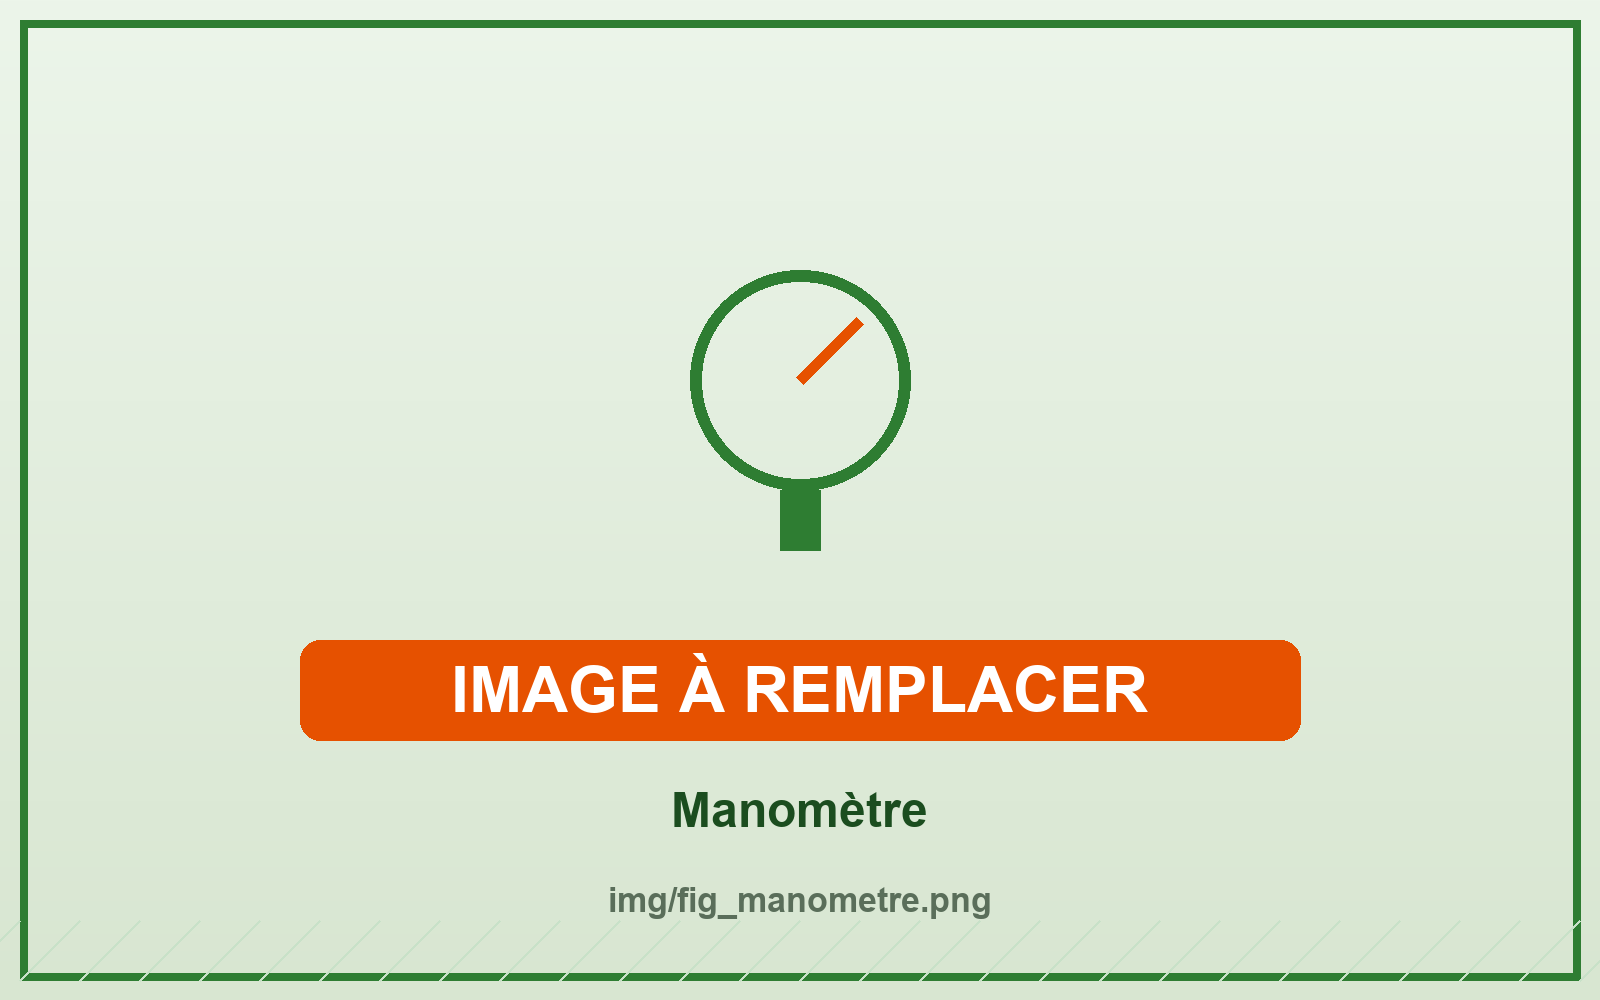
\includegraphics[width=\linewidth]{img/fig_manometre}
  \caption{manomètre}\label{fig:manometre}
\end{minipage}\hfill
\begin{minipage}{0.48\textwidth}\centering
  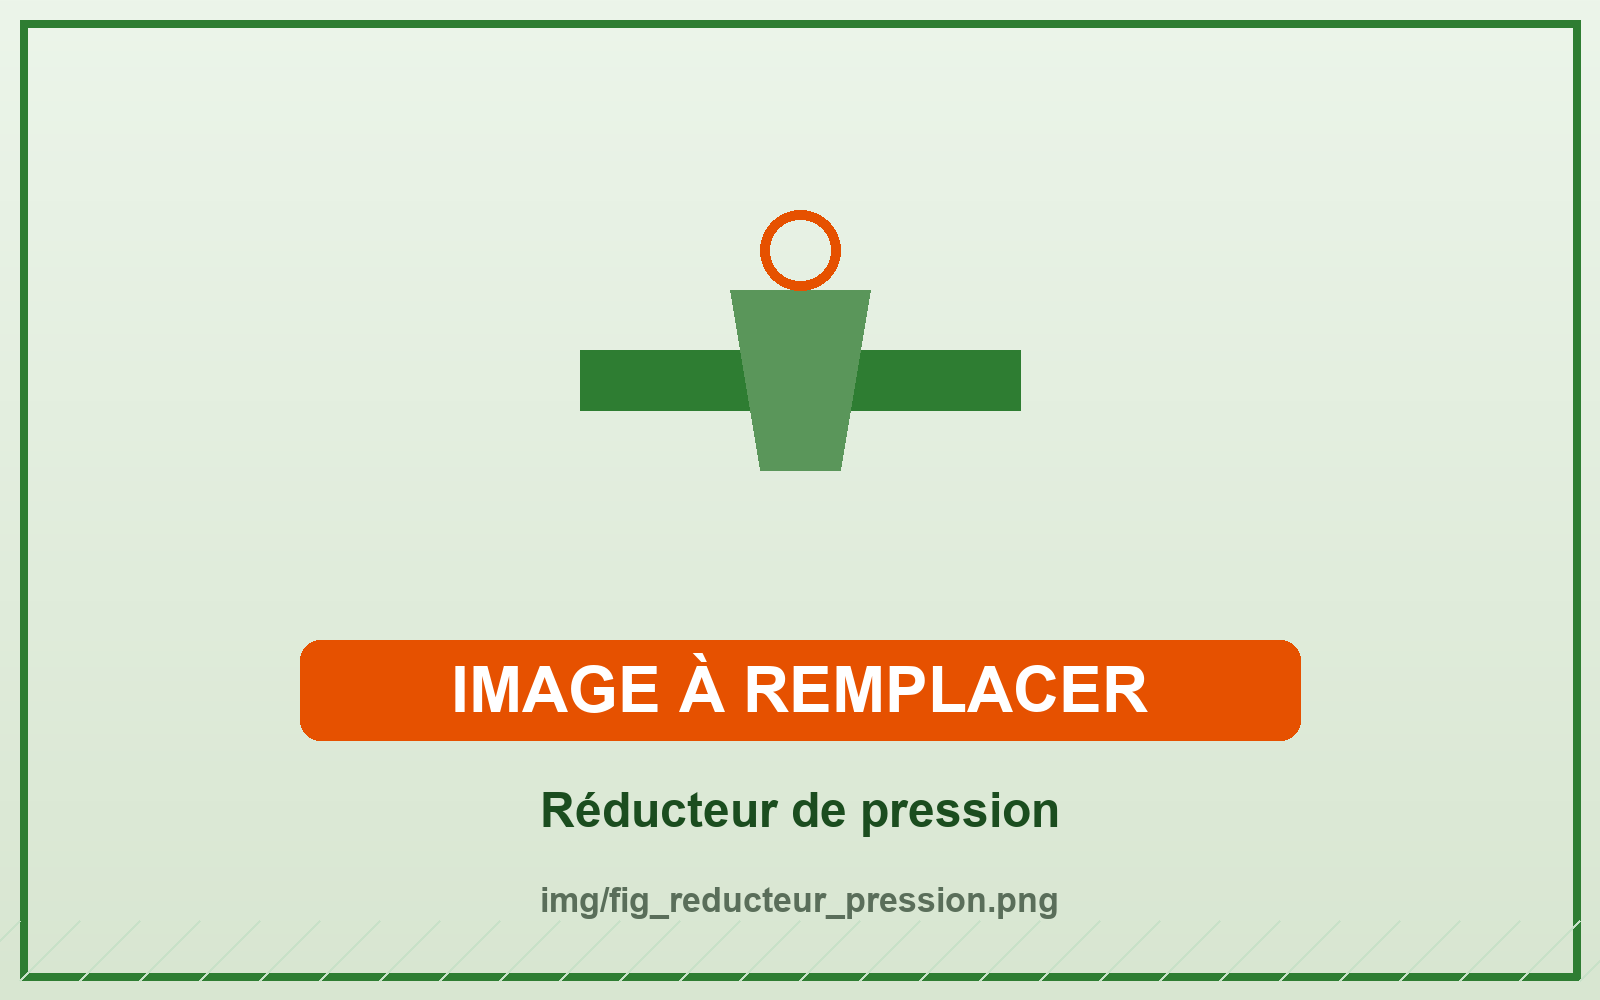
\includegraphics[width=\linewidth]{img/fig_reducteur_pression}
  \caption{réducteur de pression}\label{fig:reducteur}
\end{minipage}
\end{figure}

\begin{itemize}
  \item \textbf{Manomètre} (figure~\ref{fig:manometre}) : il indique la pression de l'eau dans
        le circuit, en bar. Monté en aval du réducteur, il permet de contrôler le réglage.
  \item \textbf{Réducteur de pression} (figure~\ref{fig:reducteur}) : il abaisse et stabilise
        la pression en aval, quelle que soit la pression amont, pour protéger la robinetterie et
        limiter la consommation.
\end{itemize}

\begin{figure}[H]\centering
\begin{minipage}{0.31\textwidth}\centering
  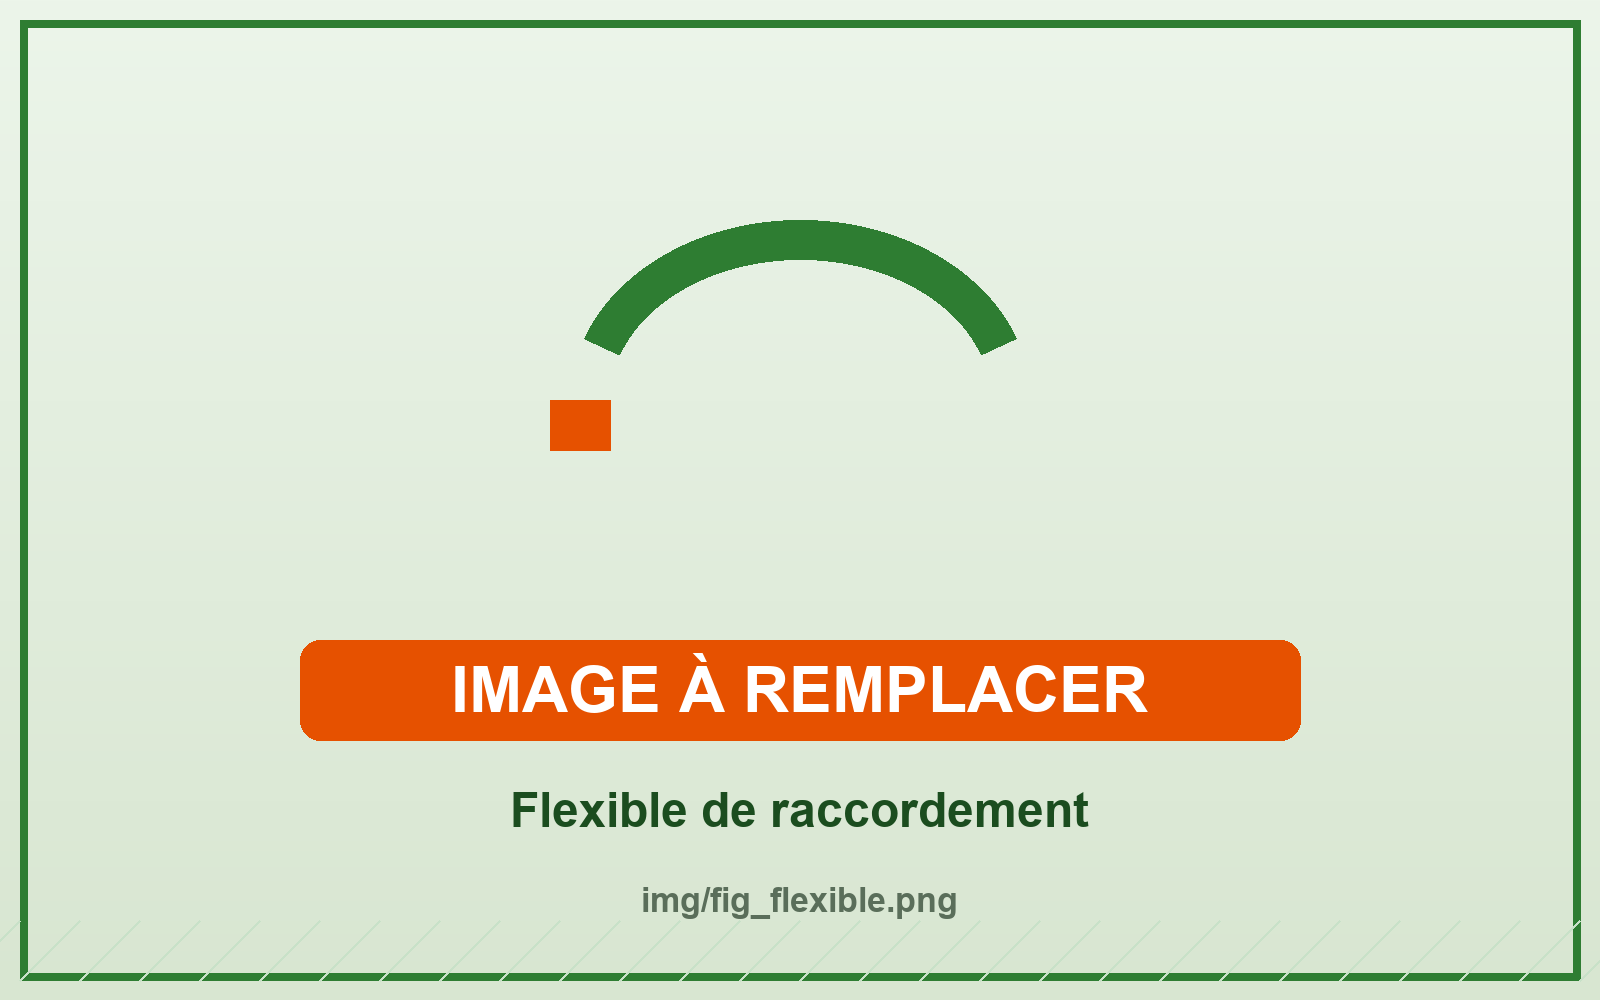
\includegraphics[width=\linewidth]{img/fig_flexible}
  \caption{flexible de raccordement}\label{fig:flexible}
\end{minipage}\hfill
\begin{minipage}{0.31\textwidth}\centering
  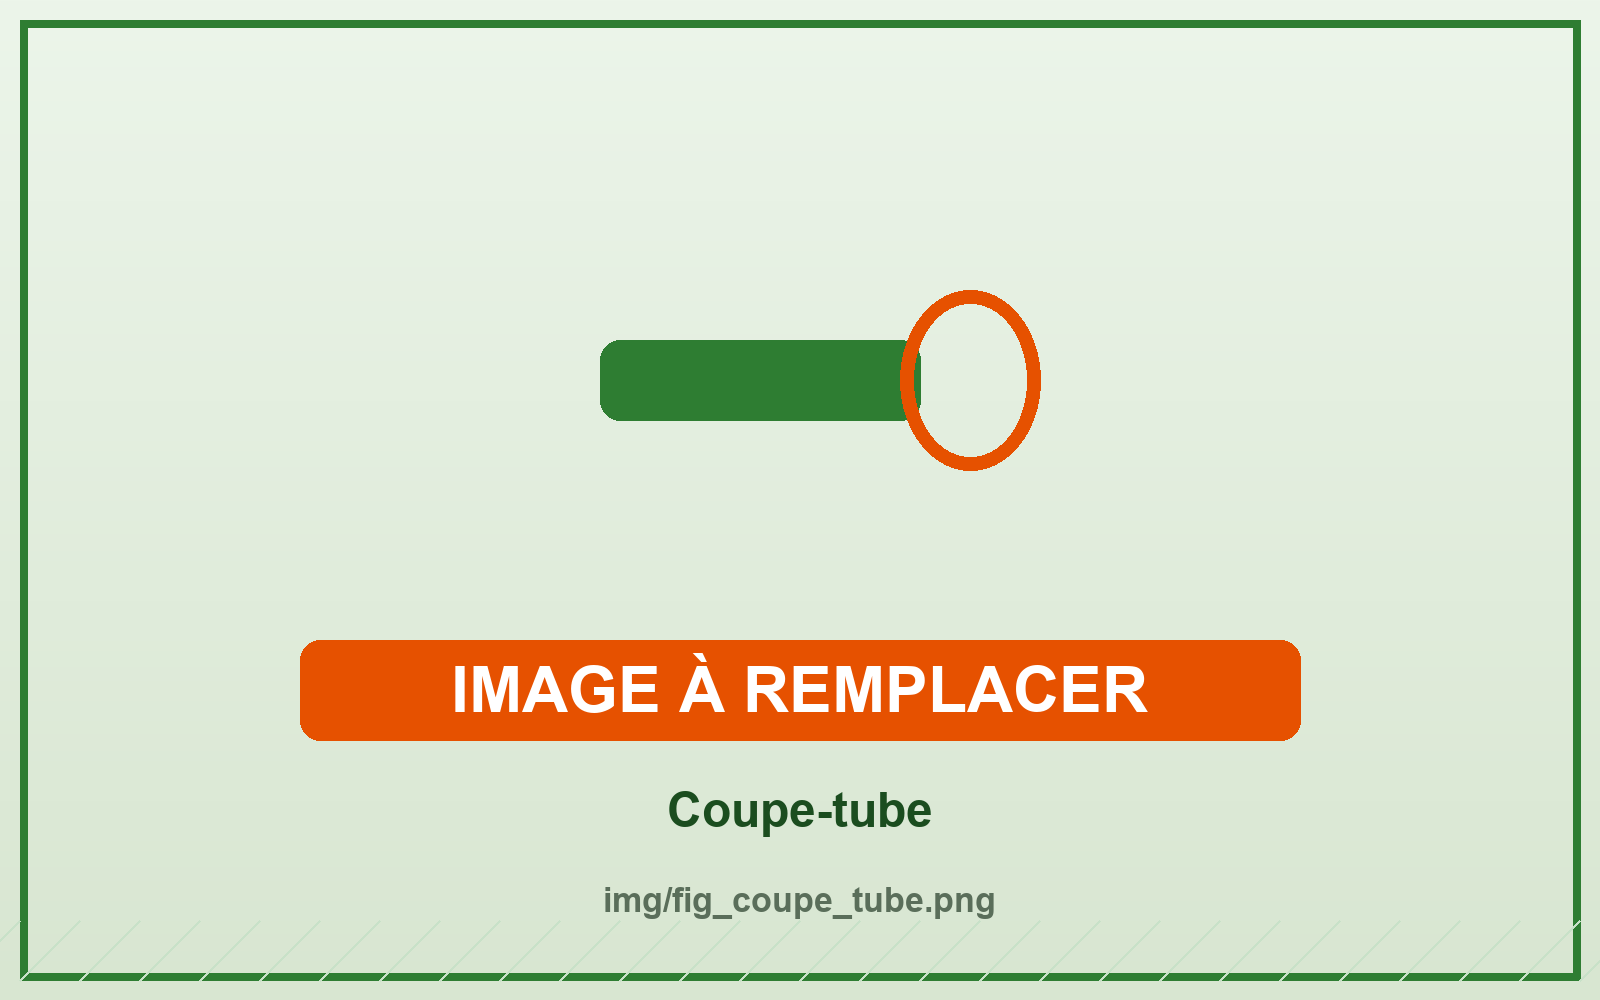
\includegraphics[width=\linewidth]{img/fig_coupe_tube}
  \caption{coupe-tube}\label{fig:coupetube}
\end{minipage}\hfill
\begin{minipage}{0.31\textwidth}\centering
  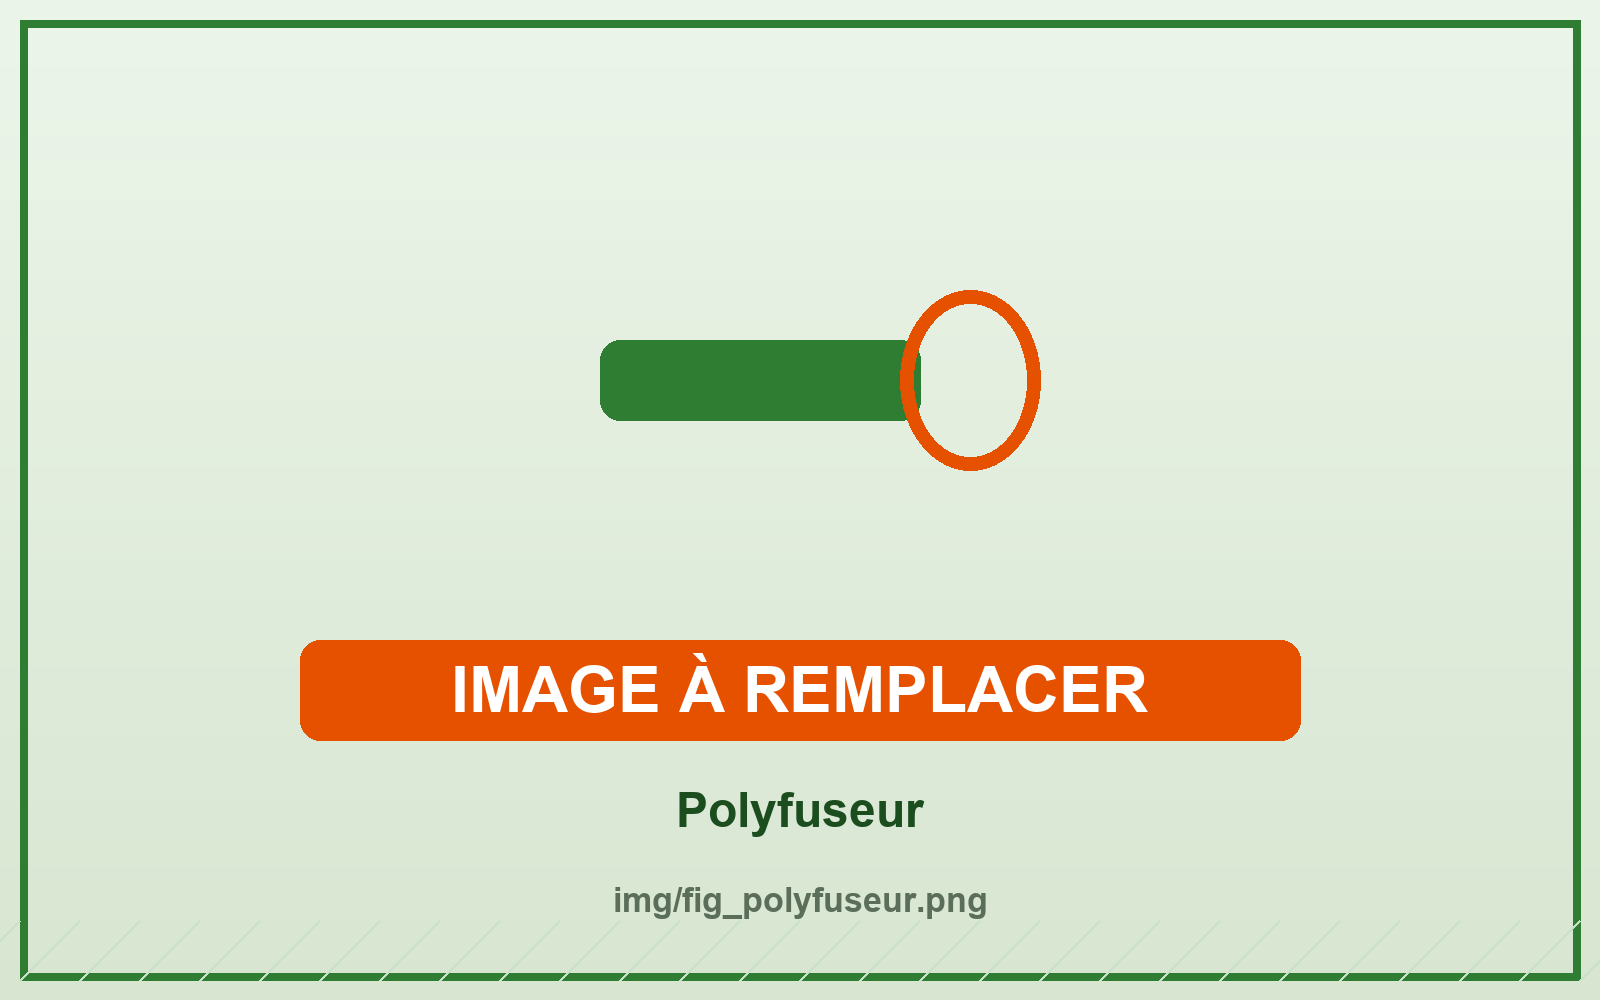
\includegraphics[width=\linewidth]{img/fig_polyfuseur}
  \caption{polyfuseur}\label{fig:polyfuseur}
\end{minipage}
\end{figure}

\begin{itemize}
  \item \textbf{Flexibles de raccordement} (figure~\ref{fig:flexible}) : en inox tressé, ils
        relient la canalisation fixe à la robinetterie des appareils.
  \item \textbf{Coupe-tube} (figure~\ref{fig:coupetube}) : il assure une coupe nette et
        perpendiculaire des tubes PPR de petit diamètre, condition d'une bonne soudure.
  \item \textbf{Polyfuseur} (figure~\ref{fig:polyfuseur}) : appareil chauffant équipé de
        matrices mâle et femelle, il permet d'assembler les tubes et raccords PPR par fusion,
        sans colle.
\end{itemize}

\section{Mise en œuvre : modes opératoires}

\subsection{Assemblage des tubes PPR par polyfusion}
La polyfusion soude le tube et le raccord en fondant simultanément leurs surfaces de contact.
La température de la matrice doit être de \SI{260}{\celsius} \cite{wavinPPR}. Le mode
opératoire est le suivant :
\begin{enumerate}
  \item monter les matrices du diamètre voulu et laisser le polyfuseur atteindre
        \SI{260}{\celsius}, en attendant quelques minutes après le voyant de température ;
  \item couper le tube d'équerre au coupe-tube, l'ébavurer et le nettoyer ;
  \item marquer sur le tube la profondeur d'emboîtement ;
  \item engager simultanément le tube et le raccord dans les matrices, sans rotation ;
  \item respecter le temps de chauffe indiqué par le fabricant pour le diamètre ;
  \item retirer les pièces et les emboîter immédiatement, sans rotation, jusqu'au repère ;
  \item maintenir l'assemblage quelques secondes, puis le laisser refroidir avant toute
        sollicitation.
\end{enumerate}
Un temps de chauffe trop court donne une soudure non étanche. Un temps trop long rétrécit le
passage intérieur par formation d'un bourrelet.

\subsection{Montage d'un réducteur de pression et d'un manomètre}
\begin{enumerate}
  \item isoler et vidanger le tronçon concerné ;
  \item repérer le sens d'écoulement indiqué par la flèche sur le corps du réducteur ;
  \item monter le réducteur entre deux vannes d'isolement, en amont de la distribution d'étage,
        avec un filtre en amont si le modèle n'en comporte pas ;
  \item assurer l'étanchéité des filetages au ruban PTFE ou à la filasse avec pâte ;
  \item visser le manomètre sur la prise prévue en aval (figure~\ref{fig:montage_reducteur}) ;
  \item remettre en eau lentement, puis régler la pression aval à la valeur prescrite
        (environ \SI{3}{bar}) en lisant le manomètre, robinets fermés.
\end{enumerate}

\figureimg{img/fig_reducteur_montage}{0.62\textwidth}{montage du réducteur de pression et du manomètre sur la distribution d'étage}{fig:montage_reducteur}

\subsection{Isolation des canalisations}
Les canalisations d'eau chaude sont isolées pour limiter les pertes de chaleur. Les
canalisations d'eau froide qui traversent des zones chaudes ou climatisées le sont pour éviter
la condensation. L'isolant utilisé est une mousse élastomère à cellules fermées (de type
Armaflex), qui forme également un pare-vapeur \cite{armacell}. Les manchons sont fendus,
posés sur le tube, puis collés à la colle néoprène sur toute la longueur de la fente et aux
jonctions, sans étirer le matériau (figure~\ref{fig:isolation}).

\figureimg{img/fig_isolation_pose}{0.62\textwidth}{pose de l'isolant à cellules fermées sur une canalisation}{fig:isolation}

\subsection{Essai d'étanchéité}
Avant de refermer les gaines et de poser les revêtements, chaque réseau est soumis à un essai
de pression conforme au NF DTU~60.1 et au cahier des charges du marché \cite{dtu601,ffbEssais}.
Sur le chantier, l'essai se déroulait ainsi :
\begin{enumerate}
  \item obturer toutes les extrémités et purger l'air du réseau ;
  \item monter en pression avec la pompe d'épreuve jusqu'à la pression d'essai prescrite ;
  \item isoler la pompe et relever la pression au manomètre ;
  \item maintenir l'essai pendant la durée prescrite, sans chute de pression ;
  \item inspecter visuellement chaque assemblage ;
  \item consigner le résultat sur la fiche d'autocontrôle (\hyperref[ann:fiche]{annexe~2}).
\end{enumerate}
La pression et la durée d'essai sont celles du cahier des charges : \AC{pression d'essai et
durée retenues sur le chantier}.

\section{Hygiène, sécurité et environnement}

Les travaux de plomberie sur un chantier de grande hauteur exposent à plusieurs risques :
chutes de hauteur, brûlures (polyfuseur à \SI{260}{\celsius}), coupures, manutention de charges
et risques électriques. Les mesures de prévention appliquées sont les suivantes :
\begin{itemize}
  \item port obligatoire des EPI : casque, chaussures de sécurité, gants, lunettes, et
        harnais pour les travaux en hauteur ;
  \item polyfuseur posé sur son support, jamais laissé sous tension sans surveillance ;
  \item escabeaux et échafaudages vérifiés avant usage ;
  \item rangement du poste de travail et évacuation quotidienne des chutes de tubes ;
  \item tri des déchets (plastiques, emballages) et récupération des chutes réutilisables.
\end{itemize}
Des photographies des EPI et du matériel d'essai figurent en \hyperref[ann:photos]{annexe~3}.

\section{Liens avec le froid et la climatisation}

Bien que le thème de ce rapport soit la plomberie sanitaire, plusieurs activités du stage
relèvent directement de notre spécialité.

\subsection{Isolation et condensation}
Lorsqu'une canalisation froide traverse un air chaud et humide, sa surface peut descendre
sous la \textbf{température de rosée} de l'air : la vapeur d'eau s'y condense, ce qui provoque
des gouttes, des taches et de la corrosion. C'est exactement le phénomène que l'on combat en
climatisation sur les lignes d'aspiration et les réseaux d'eau glacée. L'isolant à cellules
fermées maintient la surface extérieure au-dessus du point de rosée.

\subsection{Rappel du cycle frigorifique}
Les climatiseurs installés dans le bâtiment fonctionnent selon le cycle frigorifique à
compression de vapeur (figure~\ref{fig:cycle}). Le fluide frigorigène s'évapore dans
l'évaporateur en absorbant la chaleur de la pièce. Il est comprimé par le compresseur, se
condense dans le condenseur en rejetant cette chaleur à l'extérieur, puis se détend dans le
détendeur avant de revenir à l'évaporateur.

\begin{figure}[H]\centering
% Cycle frigorifique à compression de vapeur
\begin{tikzpicture}[font=\small, >=Stealth,
  org/.style={draw=vertnuit, fill=vertclair, rounded corners=3pt, align=center,
              minimum width=3.2cm, minimum height=1.1cm, font=\small\bfseries},
  hp/.style={red!75!black, line width=1.5pt, ->},
  bp/.style={blue!70!black, line width=1.5pt, ->}]
  \node[org] (cond) at (0,3) {Condenseur\\{\scriptsize\normalfont (unité extérieure)}};
  \node[org] (evap) at (0,0) {Évaporateur\\{\scriptsize\normalfont (unité intérieure)}};
  \node[org, minimum width=2.4cm] (comp) at (4.2,1.5) {Compresseur};
  \node[org, minimum width=2.4cm] (det) at (-4.2,1.5) {Détendeur};
  \draw[hp] (comp.north) |- node[pos=0.75, above] {vapeur HP, chaude} (cond.east);
  \draw[hp] (cond.west) -| node[pos=0.25, above] {liquide HP} (det.north);
  \draw[bp] (det.south) |- node[pos=0.75, below] {mélange BP, froid} (evap.west);
  \draw[bp] (evap.east) -| node[pos=0.25, below] {vapeur BP} (comp.south);
  \draw[->, orange!80!black, line width=1pt] (0,4.0) -- ++(0,0.8) node[above] {chaleur rejetée à l'extérieur};
  \draw[<-, teal, line width=1pt] (0,-0.6) -- ++(0,-0.8) node[below] {chaleur absorbée dans la pièce};
\end{tikzpicture}

\caption{cycle frigorifique à compression de vapeur}\label{fig:cycle}
\end{figure}

\subsection{Évacuation des condensats des climatiseurs}
L'eau condensée sur l'évaporateur des unités intérieures doit être évacuée. Les tuyaux de
condensats sont raccordés au réseau d'eaux usées par l'intermédiaire d'un \textbf{siphon},
qui empêche la remontée des odeurs, avec une pente régulière d'au moins 1 \%. Lors de notre
appui à l'équipe climatisation (semaine S15), nous avons participé à ces raccordements
(figure~\ref{fig:condensats}). Ils montrent concrètement l'interface entre les deux lots.

\figureimg{img/fig_condensats_split}{0.6\textwidth}{raccordement de l'évacuation des condensats d'une unité intérieure}{fig:condensats}

\subsection{Eau chaude sanitaire et pompe à chaleur}
La production d'eau chaude sanitaire peut être assurée par une \textbf{pompe à chaleur}, qui
utilise le même cycle frigorifique que le climatiseur, mais en valorisant la chaleur du
condenseur. Sur les bâtiments climatisés, la chaleur rejetée par les groupes peut même être
récupérée pour préchauffer l'eau chaude sanitaire. Cette solution réduit fortement la
consommation d'énergie.

\conclusionPartielle
La plomberie sanitaire d'un immeuble repose sur des règles précises de débit, de vitesse et de
pression. L'étude de cas montre que la colonne montante doit être dimensionnée pour le dernier
étage, et que les étages bas nécessitent des réducteurs de pression. La qualité de la mise en
œuvre (polyfusion, isolation, essais) conditionne la fiabilité de l'ouvrage. Enfin, ce thème
rejoint notre spécialité par l'isolation, les condensats et la production d'eau chaude. Ces
observations nourrissent les critiques et suggestions de la quatrième partie.

\partie{QUATRIÈME PARTIE}{CRITIQUES ET SUGGESTIONS}

% Le cours (module 2, III.3) demande une analyse critique argumentée de l'entreprise, de ses
% processus et de son organisation, et non un « documentaire léger ».

Cette partie présente un regard critique et constructif sur l'organisation du chantier et de
l'entreprise. Elle est établie à partir de nos observations. Pour chaque point, nous
proposons une piste d'amélioration réaliste.

\section{Critiques}

\subsection{Points forts constatés}
Il est juste de commencer par souligner ce qui fonctionne bien :
\begin{itemize}
  \item un \textbf{encadrement technique de qualité}, avec des chefs d'équipe expérimentés et
        disponibles pour transmettre leur savoir-faire ;
  \item une \textbf{organisation par zones} claire, qui permet de suivre l'avancement étage
        par étage ;
  \item l'usage systématique des \textbf{essais d'étanchéité} avant la fermeture des gaines,
        qui évite des reprises coûteuses ;
  \item une \textbf{bonne coordination} avec les autres lots, notamment la climatisation.
\end{itemize}

\subsection{Points à améliorer}
\begin{table}[H]\centering
\caption{constats et conséquences observés}\label{tab:critiques}
\begin{tabularx}{\textwidth}{>{\bfseries}p{3.6cm} Y Y}
\toprule
\entete Domaine & Constat & Conséquence \\
\midrule
Logistique & Ruptures ponctuelles de raccords et de consommables & Arrêts de production, réorganisation des zones \\
Sécurité du matériel & Disparitions de matériel et d'outillage sur le chantier & Surcoûts, retards, perte de temps en recherches \\
Sécurité des personnes & Port des EPI pas toujours respecté, travaux en hauteur sans protection collective & Risque d'accident grave \\
Conditions de travail & Éclairage insuffisant dans certaines gaines et cages d'escalier & Erreurs d'exécution, fatigue, perte de temps \\
Ponctualité & Démarrages tardifs de certaines équipes & Retards cumulés sur le planning \\
Traçabilité & Fiches d'autocontrôle remplies de façon irrégulière & Difficulté à prouver la qualité à la réception \\
\bottomrule
\end{tabularx}
\end{table}

Sur le plan organisationnel, l'organigramme ne prévoit pas de \textbf{responsable
hygiène-sécurité-environnement} dédié sur les grands chantiers. Ce poste nous paraît manquant
au regard des risques identifiés.

\section{Suggestions}

\begin{table}[H]\centering
\caption{suggestions d'amélioration}\label{tab:suggestions}
\begin{tabularx}{\textwidth}{>{\bfseries}p{3.6cm} Y}
\toprule
\entete Domaine & Suggestion \\
\midrule
Logistique & Établir pour chaque zone une liste de matériel prévisionnelle, avec un stock tampon des raccords courants géré par le magasinier \\
Sécurité du matériel & Fermer un local de stockage par niveau, tenir un registre des sorties d'outillage, organiser des rondes \\
Sécurité des personnes & Désigner un référent HSE, faire un quart d'heure sécurité hebdomadaire, imposer le port des EPI et installer des garde-corps \\
Conditions de travail & Installer des projecteurs de chantier et un éclairage provisoire dans les gaines \\
Ponctualité & Fixer une heure de briefing quotidien de 10 minutes pour lancer la journée \\
Traçabilité & Généraliser les fiches d'autocontrôle signées par le chef d'équipe, avec photos des essais \\
Formation & Former tout le personnel au soudage PPR et aux bonnes pratiques d'isolation \\
\bottomrule
\end{tabularx}
\end{table}

\conclusionPartielle
L'entreprise dispose d'atouts réels : un savoir-faire technique reconnu et une organisation
claire. Les axes de progrès concernent surtout la logistique, la sécurité et la traçabilité.
Les suggestions proposées sont peu coûteuses et pourraient améliorer à la fois la
productivité, la sécurité du personnel et l'image de l'entreprise auprès de ses clients.

\pageTitre{CONCLUSION}

Au terme de ces \InfoDuree{} de stage au sein de \InfoEntreprise, le bilan est largement
positif. Nous avons découvert le fonctionnement d'une entreprise de lots techniques du bâtiment
et participé, au sein de l'équipe plomberie, à la réalisation des réseaux d'eau froide et
d'eau chaude sanitaire du chantier \InfoChantier. Nous y avons acquis des gestes
professionnels concrets : assemblage du PPR par polyfusion, montage et réglage des
réducteurs de pression, isolation des canalisations et essais d'étanchéité.

Sur le plan technique, l'étude de cas a montré comment les règles du NF DTU~60.11 permettent
de dimensionner une colonne montante et de justifier la pose de réducteurs de pression aux
étages bas. Elle illustre le lien direct entre la théorie vue en formation et les choix faits
sur le chantier. Ce stage a répondu à nos attentes : il nous a fait progresser en rigueur, en
autonomie et en travail d'équipe, et notre implication a été appréciée par l'encadrement.

Ce travail comporte toutefois des \textbf{limites}. Notre participation s'est concentrée sur la
distribution d'eau : nous n'avons pas travaillé sur les évacuations ni sur la mise en service
complète du surpresseur. L'étude de cas repose sur des hypothèses simplifiées et devrait être
confirmée par la note de calcul du bureau d'études. Il serait intéressant de prolonger cette
étude par l'analyse des réseaux d'évacuation et par un bilan énergétique de la production
d'eau chaude, comparant chauffe-eau électriques et pompe à chaleur.

Nous recommandons à l'entreprise de renforcer sa logistique, sa politique de sécurité et la
traçabilité de ses autocontrôles. Aux futurs stagiaires, nous recommandons de prendre des notes
chaque jour et de ne pas hésiter à poser des questions.

Enfin, ce stage a conforté notre \textbf{projet professionnel} : devenir technicien en froid et
climatisation, capable d'intervenir également sur les réseaux de fluides du bâtiment. La
proximité entre ces métiers, constatée sur le terrain, est un atout que nous comptons valoriser
dans notre insertion professionnelle.


% ------------------------------------------------------------- Bibliographie
\pageTitre{BIBLIOGRAPHIE}
\nocite{coursModule2}
\printbibliography[heading=none]

% ------------------------------------------------------------------- Annexes
\pageTitre{ANNEXES}

% Règle du cours : chaque annexe est annoncée dans le corps du rapport par un renvoi.

\section*{Annexe 1 : schéma d'une installation sanitaire de logement}\label{ann:schema}
\addcontentsline{toc}{section}{Annexe 1 : schéma d'une installation sanitaire de logement}
Ce schéma complète la figure~\ref{fig:principe} de la troisième partie à l'échelle d'un
logement.

\begin{figure}[H]\centering
% Logement type : compteur -> réducteur -> nourrices EF/ECS -> appareils
\begin{tikzpicture}[font=\scriptsize, >=Stealth,
  eq/.style={draw=vertnuit, fill=vertclair, rounded corners=2pt, align=center, minimum height=7mm, inner sep=2pt},
  app/.style={draw=gray!70, fill=white, align=center, minimum width=14mm, minimum height=6mm},
  ef/.style={blue!70!black, line width=1.1pt, ->},
  ecs/.style={red!75!black, line width=1.1pt, ->}]
  \node[eq] (v1) at (0,0) {Vanne\\d'arrêt};
  \node[eq, right=5mm of v1] (cpt) {Compteur};
  \node[eq, right=5mm of cpt] (cl) {Clapet\\anti-retour};
  \node[eq, right=5mm of cl, fill=acompleter!15] (red) {Réducteur\\de pression};
  \node[eq, right=5mm of red] (nef) {Nourrice EF};
  \draw[ef] (v1) -- (cpt); \draw[ef] (cpt) -- (cl); \draw[ef] (cl) -- (red); \draw[ef] (red) -- (nef);
  \node[eq, below=14mm of red, fill=red!10] (ce) {Chauffe-eau};
  \node[eq, right=5mm of ce] (necs) {Nourrice ECS};
  \draw[ef] (red.south) -- (ce.north);
  \draw[ecs] (ce) -- (necs);
  \foreach \a/\x/\n in {Lavabo/11.0/a, Douche/12.4/b, WC/13.8/c, Évier/15.2/d} {
    \node[app] (A\n) at (\x,-0.9) {\a};
  }
  \draw[blue!70!black, line width=1.1pt] (nef.east) -- ++(0.3,0) -- ++(0,0.5);
  \foreach \n in {a,b,c,d} \draw[ef] (nef.east) ++(0.3,0.5) -| (A\n.north);
  \draw[ecs] (necs.east) -| (Aa.south);
  \draw[ecs] (necs.east) -| (Ab.south);
  \draw[ecs] (necs.east) -| (Ad.south);
  \node[anchor=west, text width=6cm] at (0,-3.2) {Distribution en tube PPR (ou PER) depuis les nourrices :
     une canalisation par appareil, sans raccord intermédiaire en partie encastrée.};
\end{tikzpicture}

\caption{schéma d'une installation sanitaire de logement (distribution en nourrice)}\label{fig:logement}
\end{figure}

\clearpage
\section*{Annexe 2 : fiche d'autocontrôle de l'essai d'étanchéité}\label{ann:fiche}
\addcontentsline{toc}{section}{Annexe 2 : fiche d'autocontrôle de l'essai d'étanchéité}
Modèle de fiche utilisé pour consigner les essais (voir troisième partie, essai d'étanchéité).

\begin{center}
\renewcommand{\arraystretch}{1.6}
\begin{tabularx}{\textwidth}{|>{\bfseries}p{5cm}|X|}
\hline
\rowcolor{vertclair} \multicolumn{2}{|c|}{\textbf{FICHE D'AUTOCONTRÔLE -- ESSAI D'ÉTANCHÉITÉ}} \\ \hline
Chantier & \InfoChantier \\ \hline
Niveau / zone & \\ \hline
Réseau testé (EF / ECS) & \\ \hline
Date et heure de début & \\ \hline
Pression d'essai (bar) & \\ \hline
Pression en fin d'essai (bar) & \\ \hline
Durée de l'essai & \\ \hline
Résultat (conforme / non conforme) & \\ \hline
Observations et reprises & \\[1.5cm] \hline
Nom et visa du technicien & \\ \hline
Nom et visa du chef d'équipe & \\ \hline
\end{tabularx}
\end{center}

\clearpage
\section*{Annexe 3 : photographies complémentaires du chantier}\label{ann:photos}
\addcontentsline{toc}{section}{Annexe 3 : photographies complémentaires du chantier}

\figureimg{img/fig_epi_chantier}{0.6\textwidth}{équipements de protection individuelle portés sur le chantier}{fig:epi}
\figureimg{img/fig_essai_etancheite}{0.6\textwidth}{pompe d'épreuve raccordée pour un essai d'étanchéité}{fig:essai}


% --------------------------------------------------------- Table des matières
\clearpage\phantomsection
\addcontentsline{toc}{chapter}{TABLE DES MATIÈRES}
\etocsettocstyle{\banniere{TABLE DES MATIÈRES}\vspace{0.4em}}{}
\etocsetnexttocdepth{subsubsection}
\tableofcontents

\end{document}
